\section{Klasické šifry}
V tejto kapitole sa budeme zaoberať históriou a stručným prehľadom klasických šifier.
Spomenieme si aj niektoré základné útoky na klasické šifry. 

\subsection{História}
História klasických šifier a utajovania písomného textu je pravdepodobne tak stará ako samotné písmo.
Písmo, v podobe akej ho poznáme a používame dnes, pravdepodobne pochádza asi spred 3000 rokov pred Kristom a za jeho objaviteľov sa považujú
Feničania.
V niektorých prípadoch predstavovalo už použitie písma utajenie samotného textu.
Príkladom môžu byť Egyptské hieroglyfy alebo klinové písmo používané v Mezopotámii.
Iným príkladom môžu byť semitské jazyky, ktoré sú charakteristické používaním iba spoluhlások bez použitia samohlások,
pretože tie zaviedli až Aremejci a po nich následné Gréci, aby pomocou nich boli schopný rozlíšiť jazyky \cite{ks}.
Aj diakritika ako taká má schopnosť rozlišovať významy slov, čo si ale až do 15.storočia nikto nevšímal,
až pokiaľ ju Arabi nezačali používať pri kryptoanalýze rôznych šifier.

Z historického hľadiska nie je možné presne zoradiť ako jednotlivé šifry vznikali, pretože súčasne vznikali na viacerých miestach sveta.
Komunikácia a s ňou spojené sírenie informácií nebolo také rýchle ako dnes, až do roku 1440, keď Johan Guttenberg vynašiel kníhtlač,
čo zjednodušilo výmenu a uchovávanie informácií.
% (TODO: pridať utajovanie informácie)

Ku kryptografii ako aj k rôznym iným vedným disciplínam prispelo v minulosti staré Grécko.
Jedným z najvýznamnejších príspevkov starých Grékov bolo široké rozšírenie abecedy a písomného prejavu.
Gréci písmo prebrali od Feničanov, ktorí na rozdiel od Egypťanov používali jednoduchšie písmo.

V Európe vďaka rozšíreniu abecedy začali vznikať aj prvé šifry, medzi ktoré patrí napríklad Cézarova šifra, ktorá vznikla v Rímskej ríši.
Iným príkladom môže byť transpozičná šifra skytalé, ktorá bola používaná v Sparte.

Pád Rímskej ríše spôsobil úpadok kryptografie, ktorý trval až do obdobia stredoveku. Typickým znakom kryptografie v tomto období bolo
napríklad písanie odzadu, alebo vertikálne, používanie cudzích jazykov, alebo vynechávanie samohlások \cite{ks}.

V stredoveku, kvôli bojom medzi pápežmi Ríma a Avignonu, bola kryptografia zdokonalená a začali sa používať rôzne kódy a nomenklátory.
Ich charakteristickým znakom bolo zamieňanie písmen alebo nahradzovanie mien a titulov osôb v správach.
V tomto období zabezpečovanie utajenia správ pokročilo až na takú úroveň, že na doručovanie správ boli použitý špeciálne vycvičení kuriéri.

V prvej polovici 20. storočia ľudia, ktorí pracovali v oblasti utajovanej komunikácie verili, že na to, aby bola zabezpečená utajovaná komunikácia musí byť utajený kľúč a okrem neho aj šifrovací algoritmus. Toto ale odporovalo Kerckhoffovmu princípu, ktorý hovorí že: \textquote{Bezpečnosť šifrovacieho algoritmu musí závisieť výlučne na utajení kľúča a nie algoritmu}. Okrem toho sformuloval aj niekoľko požiadaviek na kryptografický systém, medzi ktoré patria:
\begin{enumerate}
\item systém musí byť teoreticky, alebo aspoň prakticky bezpečný
\item narušenie systému nesmie priniesť ťažkosti odosielateľovi a adresátovi
\item kľúč musí byť ľahko zapamätateľný a ľahko vymeniteľný
\item zašifrovaná správa musí byť prenášateľná telegrafom
\item šifrovacia pomôcka musí byť ľahko prenosná a ovládateľná jedinou osobou
\item systém musí byť jednoduchý, bez dlhého zoznamu pravidiel, nevyžadujúci nadmerné sústredenie
\end{enumerate}
Tieto princípy sú popísané v pôvodnej publikácii od Kerckhoffa \cite{kerckhoff}.

Existovala ale aj iná skupina vedcov, medzi ktorých patril aj Lester S. Hill, ktorý si uvedomoval, že kryptológia je úzko spätá z matematikou.
V roku 1941 si na Hillových prácach zakladal A. Adrian Albert, ktorý pochopil, že v šifrovaní je možné použiť viacero algebraických štruktúr.
Neskôr toto všetko usporiadal a zdokonalil Claude E. Shannon, čo možno považovať za ukončenie éry klasických šifier \cite{ks}.

% \todo{Možno pridať/spomenúť steganografiu.}

\subsection{Charakteristika}
Na rozdiel od moderných šifier, ktoré sa používajú dnes, sú tie klasické rozdielne v niektorých hlavných črtách.
Môžeme spomenúť niekoľko:
\begin{itemize}
\item Šifrovanie a dešifrovanie klasickej šifry možno realizovať zväčša pomocou papiera a ceruzky alebo nejakej mechanickej pomôcky.
\item V dnešnej dobe aj vďaka rozšírenému použitiu počítačov stratila väčšina týchto algoritmov svoj význam.
\item Utajuje sa algoritmus a aj kľúč a neuplatňuje sa Kerckhoffov princíp.
\item Na rozdiel od moderných šifier sa používajú malé abecedy.
\item V klasických šifrách je otvorený text, zašifrovaný text a kľúč v abecede reálneho jazyka, pričom v moderných šifrách sa používa binárne kódovanie.
\item Na klasické šifry sa zväčša dá použiť štatistická analýza. 
\end{itemize}
Zo spomenutých charakteristík existujú aj výnimky. Napríklad pri Vigenerovej šifre sa algoritmus neutajoval. To platí aj pre Vernamovu šifru, ktorá okrem toho používa navyše binárne znaky. Vernamova šifra je perfektne bezpečná v podľa Shannonovej teórie \cite{ks}.

Klasické šifry môžeme rozdeliť do niekoľkých základných kategórii:
\begin{itemize}

\item \textbf{Substitučné šifry.}
  V prípade že šifra permutuje znaky zdrojovej abecedy, hovoríme o monoalfabetickej šifre.
  Ako príklad môžeme uviesť šifru Atbaš prípadne Cézarovu šifru, alebo iné.
  V inom prípade ak sa aplikuje viacero permutácii podľa polohy znaku v otvorenom texte, tak hovoríme o polyalfabetickej šifre.
  Príkladom je Vigenerova šifra. Ďalším prípadom je polygramová šifra, kde sa z otvoreného textu najprv vytvoria bloky,
  na ktoré sa potom aplikuje nejaká permutácia.

\item \textbf{Transpozičné šifry.}
  Transpozičné šifry sú vlastne blokové šifry, ktoré pri šifrovaní a dešifrovaní aplikujú pevne zvolenú permutáciu na každý blok
  otvoreného/zašifrovaného textu. Od polyalfabetickej šifry sa líši v poradí vykonávania operácií.
  
\item \textbf{Homofónne šifry.}
  Homofónne šifry sú šifry, ktoré majú znáhodnený zašifrovaný text. Tieto šifry sa snažia zabrániť frekvenčnej analýze textu. 
  
\item \textbf{Substitučno-permutačné šifry.}
  Ak aplikujeme viacero substitučný a permutačných šifier na otvorený text tak hovoríme o substitučno-permutačných šifrách.
  Šifrovanie prebieha tak, že sa blok otvoreného textu rozdelí na menšie bloky, na ktoré je potom aplikovaná substitúcia, a permutácia,
  ktorá sa aplikuje na celý blok. Substitúcia zabezpečuje konfúziu a permutácia difúziu.
  
\end{itemize}

\subsection{Počítačové lúštenie klasických šifier}
Počítače a lúštenie šifier sú v dnešnej dobe neoddeliteľnou súčasťou. Výkon počítačov vplyvom Mooreovho zákona \footnote{Moorov zákon je empirické pravidlo, ktoré hovorí že zložitosť integrovaných obvodov sa zdvojnásobuje každých 18 až 24 mesiacov, pričom cena ostáva konštantná.} neustále narastá,
čo má za následok vznik nových metód, ktoré sa snažia využiť dostupný výkon.

\textquote{Výpočtový výkon súčasných počítačov môže byť použitý na vykonanie čiastočnej, alebo až úplnej kryptoanlýzy klasických šifier} \cite{ks}.
Takúto automatizovanú kryptoanalýzu môžeme rozdeliť do troch kategórii:
\begin{enumerate}
\item
Prvou kategóriou je počítačom asistovaná kryptoanalýza, pri ktorej lúštiteľ využíva
počítač ako pomôcku na zjednodušenie niektorých úkonov.
\item
Druhou kategóriou je poloautomatická krytoanalýza, pri ktorej počítač prehľadáva priestor riešení, avšak
rozhodujúce kroky sú prenechané na kryptoanalytika.
\item
Poslednou treťou kategóriou je automatická kryptoanalýza, pri ktorej lúštiteľ zadá zašifrovanú správu počítaču a ten mu následne poskytne jednu, prípadne aj
viac najlepších riešení.
\end{enumerate}
Automatickou kryptoanalýzou sa budeme zaoberať aj v tejto práci.
Pri automatickej kryptoanalýze zohráva veľkú úlohu analýza a ohodnocovanie textov, pretože niektoré spôsoby lúštenia šifier,
napríklad útok hrubou silou, produkujú veľké množstvo možných riešení, ktoré treba nejakým spôsobom ohodnotiť.

Na automatické ohodnocovanie textov sa používa ohodnocovacia funkcia, pomocou ktorej môžeme stanoviť určitý stupeň kvality, takzvané skóre.
Podľa skóre potom môžeme niektoré texty zahodiť a iné posunúť na ďalšie posúdenie.
Jednoduchú ohodnocovaciu funkciu by sme mohli skonštruovať napríklad pomocou slovníka.
Existujú ale aj iné metódy, lepšie metódy, napríklad n-gramy, ktoré využívajú frekvencie dvojíc, trojíc, n-tíc znakov jazyka.

Pri vhodne zvolenej ohodnocovacej funkcii začnú vznikať v priestore riešení takzvané extrémy. Na to aby sme v priestore riešení našli globálny extrém,
nepotrebujeme prehľadať všetky riešenia. Existujú algoritmy, ktoré dokážu nájsť globálny extrém rýchlejšie.
Medzi takéto algoritmy patria napríklad: horolezecký algoritmus, simulované žíhanie, genetické algoritmy, a iné.

\subsubsection{Útok hrubou silou}
Útok hrubou silou (bruteforce) je typ útoku, ktorý sa snaží zlomiť kľúč tak, že sa prehľadáva celý priestor kľúčov.
Aby bol takýto útok možný a prakticky realizovateľný, priestor prehľadávaných kľúčov nesmie byť väčší ako hranica daná dostupnými
prostriedkami alebo časom potrebným na riešenie.

Pre ilustráciu si uveďme jednoduchý príklad. Majme zašifrovaný text \textquote{VECDOXSORSCDYBSMUIMRCSPSOBXKQBSNO}, ktorý vieme že bol zašifrovaný šifrou podobnou Cézarovej šifry.
Pre získanie otvoreného textu potrebujeme vyskúšať všetkých 26 možností posunov, čo je v tomto prípade kľúč, tak, aby sme dostali zmysluplný text.

\begin{lstlisting}
kluc 1
VECDOXSORSCDYBSMUIMRCSPSOBXKQBSNO
WFDEPYTPSTDEZCTNVJNSDTQTPCYLRCTOP

kluc 2
VECDOXSORSCDYBSMUIMRCSPSOBXKQBSNO
XGEFQZUQTUEFADUOWKOTEURUQDZMSDUPQ

kluc 3
VECDOXSORSCDYBSMUIMRCSPSOBXKQBSNO
YHFGRAVRUVFGBEVPXLPUFVSVREANTEVQR

... // dalsie kluce 4..26
\end{lstlisting}

Po prezretí všetkých možností by sme zistili že kľúč 16 sa dešifruje na \textquote{LUSTENIEHISTORICKYCHSIFIERNAGRIDE}.

% \todo{praktickosť útoku}

\subsubsection{Slovníkový útok}
Slovníkový útok narozdiel od útoku hrubou silou skúša iba niektoré možnosti z vopred pripraveného slovníka kľúčov.

Ukážme si ako by v princípe mohol fungovať slovníkový útok na šifru Vigenere.
Nech zašifrovaný text je \textquote{SYKESUMWSWZXGCWJOQNVZMXTSYRSRFPHW}. Útočník má k dispozícii slovník slov \textquote{ABC, SOMAR, HESLO, ...}.

\begin{lstlisting}
kluc: JANO
SYKESUMWSWZXGCWJOQNVZMXTSYRSRFPHW
JYXQJUZIJWMJXCJVFQAHQMKFJYEEIFCTN

kluc: SOMAR
SYKESUMWSWZXGCWJOQNVZMXTSYRSRFPHW
AKYEBCYKSFHJUCFRAENEHYLTBGDGROXTK

kluc: HESLO
SYKESUMWSWZXGCWJOQNVZMXTSYRSRFPHW
LUSTENIEHISTORICKYCHSIFIERNAGRIDE
\end{lstlisting}

\subsubsection{Horolezecký algoritmus}
Horolezecký algoritmus patrí medzi základné optimalizačné algoritmy.
Jeho základnou myšlienkou je, že na vrchol kopca sa môžeme dostať najkratšou cestou, keď pôjdeme vždy najstrmším smerom nahor.

Algoritmus sa na začiatku vždy inicializuje náhodným kľúčom. Následne sa vygeneruje množina nových potencionálnych kandidátov na riešenie
pomocou základných zmien. Ak je kľúč napríklad permutácia zmenou môže byť výmena dvoch prvkov v kľúči.
Jednotlivým kľúčom je potom priradené skóre pomocou ohodnocovacej funkcie.
Za aktuálny kľúč sa bude považovať ten, ktorý má najlepšie skóre.
Výsledky tohto algoritmu ovplyvňuje voľba ohodnocovacej funkcie, ktorá sa ľahko môže ostať v lokálnom extréme, z ktorého sa nevie dostať.

\subsubsection{Genetické algoritmy}
\acrfull{ga} patria medzi najčastejšie používaných predstaviteľov evolučných výpočtových techník.
Genetické algoritmy sa snažia napodobniť biologické procesy v prírode.

Základnými objektami sú gén, reťazec a populácia. Nad týmito objektami sa vykonávajú operácie.
Medzi základné operácie patria výber, mutácia a kríženie.

\paragraph{Gén} je základnou stavebnou jednotkou reťazca a predstavuje elementárne vlastnosti jedinca.
Gén je zvyčajne reprezentovaný číselne, alebo nejakým symbolom z abecedy.

\paragraph{Reťazec (chromozóm)} je postupnosť génov, respektíve znakov, ktoré predstavujú zvolené parametre alebo vlastnosti jedinca
z problémovej oblasti. V tomto prípade reťazec predstavuje dešifrovací kľúč. 

\paragraph{Populácia} je skupina reťazcov zvoleného počtu. Veľkosť populácie sa počas riešenia genetického algoritmu môže meniť.

\paragraph{Generácia} predstavuje populáciu GA v niektorej výpočtovej fáze, prípadne môže reprezentovať poradové číslo cyklu.

\paragraph{Účelová funkcia} vypočítava skóre každého jedinca v populácii a je mierou toho, čo chceme maximalizovať, prípadne minimalizovať.
Úlohou účelovej funkcie je nájsť globálny extrém.

\paragraph{Fitness} je v evolučných výpočtoch pojem predstavujúci mieru úspešnosti jedincov.
V prípade maximalizačnej úlohy je to najväčšia hodnota účelovej funkcie. Naopak, v prípade minimalizačnej úlohy je to najmenšia hodnota.

\paragraph{Výber} je proces, ktorý vyberie niektorých jedincov z populácie na základe zvolenej stratégie.
Vybraný jedinci potom vstupujú do operácii kríženia, mutácie alebo bez zmeny pokračujú do ďalšej generácie.
Existuje viacero stratégii výberu jedincov, avšak základnou ideou je aby lepší jedinci prežili a postupne vytlačili slabších jedincov z populácie.

\paragraph{Mutácia} znamená náhodnú zmenu génu v reťazci, prípadne viac zmien v celej populácii.
Gén zmení svoju hodnotu na inú, náhodne zvolenú hodnotu z prehľadávaného priestoru.
Mutácia je základnou hybnou silou genetických algoritmov. Umožňuje nachádzať nové riešenia, ktoré sa v populácii ešte neobjavili.

\paragraph{Kríženie} je operácia, pri ktorej si dva náhodne zvolené rodičovské jedince rozdelia v nejakom bode a vymenia si svoje gény.
Krížením vznikajú noví, odlišní potomkovia, ktorí nesú niektoré znaky oboch rodičov.

Skôr než sa GA začne realizovať treba definovať treba určiť spôsob zakódovania parameterov jednotlivých objektov.
Pri klasických šifrách sa gény zvyčajne reprezentujú pomocou abecedných znakov alebo čísiel.
Ďalším krokom je určiť prehľadávaný priestor a následne formulovať účelovú funkciu. Dôležité je aj určiť veľkosť populácie,
ktorá sa doporučuje medzi 10 a 100 jedincov \cite{ev}.
Pri malých populácia býva nedostatočný priestor pre rôznorodosť (diverzitu) genetických informácii,
naopak pri veľkých populáciách sa už nedosahuje lepšieho efektu.

\begin{figure}[!h]
  \centering
%  \def\svgwidth{\columnwidth}
  \input{ga.pdf_tex}
  \caption{Štruktúra GA}
  \label{img:ga}
\end{figure}


Princíp genetických algoritmov možno vidieť aj na obrázku \ref{img:ga}, ktorý pozostáva z niekoľkých krokov:
\begin{enumerate}
\item
  Prvým krokom je vygenerovanie počiatočnej populácie $ P_0 $.
\item
  V tomto kroku sa vyhodnocuje populácia pomocou účelovej funkcie pre aktuálnu populáciu $ P_k $.
\item
  V tejto fáze sa testuje ukončujúce podmienky genetického algoritmu.
  V prípade že algoritmus skončil vyberie za najlepší jedinec aktuálnej populácie, ktorý predstavuje výsledné riešenie GA.
\item
  Ak algoritmus ešte neskončil, nasleduje výber dvoch skupín jedincov. Najprv sa vyberie jeden, prípadne viac najlepších jedincov, ktorí sa bez zmeny skopírujú
  do novej populácie (skupina $ A $). Tieto reťazce zabezpečia monotónnu konvergenciu, čo znamená, že úloha v ďalšom kroku nebude mať horšie výsledky ako v tom predchádzajúcom.
  Ďalšie jedine vybraté iným spôsobom sú skopírované do operácie kríženia (skupina $ B $).
\item
  V operácii kríženia sa náhodne spárujú rodičovské reťazce so skupiny $ B $, s ktorých vznikne rovnaký počet potomkovských reťazcov.
  Potomkovia vytvoria skupinu $ C $, ktorá pokračuje do operácie mutácie. 
\item
  Mutácia spôsobí, že náhodne zvoleným jedincom zmenia niektoré náhodne zvolené gény a vznikne populácia $ D $.
\item
  Nová populácia $ P_{k+1} $ vzniká zjednotením populácii $ A \cup D $. Genetický algoritmus pokračuje bodom 2.
\end{enumerate}
Predstavená schéma je len príklad ako by GA mohol vyzerať, v skutočnosti však môžeme uvažovať o viacerých kritériách, ktoré vplývajú na GA.
Niektoré uvedieme v experimentálnej časti tejto práce.

\section{Grid}
Jedným z cieľov práce je preskúmať možnosti aplikovania útokov na klasické šifry v gridovom prostredí.
Grid môžeme chápať ako skupinu počítačov, uzlov, spojenú pomocou siete \acrfull{lan}, prípadne inou sieťovou technológiou,
ktoré môžu ale nemusia byť geograficky oddelené.
Účelom takýchto počítačov je poskytnúť veľký výpočtový výkon, ktorý je použitý na riešenie špecifických úloh.

\subsection{hpc.stuba.sk}
Vrámci Slovenskej technickej univerzity (STU), Centra výpočtovej techniky (CVT) sa nachádza superpočítač IBM iDataPlex, ktorý pozostáva z 52 výpočtových uzlov.
Každý výpočtový uzol má nasledovnú konfiguráciu:
\begin{itemize}
\item \acrshort{cpu}: 2 x 6 jadrový Intel Xeon X5670 2.93 GHz
\item \acrshort{ram}: 48GB (24GB na procesor)
\item \acrshort{hdd}: 2TB 7200 RPM SATA
\item \acrshort{gpu}: 2 x NVIDIA Tesla M2050 448 cuda jadier, 3GB ECC \acrshort{ram}
\item Operačný systém: Scientific Linux 6.4
\item Sieťové pripojenie: 2 x 10Gb/s Ethernet
\end{itemize}
Spolu máme k dispozícii 624 \acrshort{cpu}, 3584 cuda jadier, 2,5TB \acrshort{ram} , 104TB lokálneho úložného priestoru a ďalších 115TB zdielaného úložiska.
Výpočtový výkon dosahuje 6,76 TFLOPS a maximálny príkon aj spolu s chladením je 40kW \cite{hpc}.

kód

V tabuľke \ref{tab:filesystem} môžeme vidieť dostupné diskové umiestnenia pre každého používateľa, prípadne úlohu.
Umiestnenie \texttt{/home/\$USER} je domovským priečinkom každého používateľa.
Jedno z obmedzení tohto umiestnenia je, že môže obsahovať maximálne osemdesiattisíc súborov a priečinkov.
Taktiež má značne obmedzenú kapacitu čo sa nemusí hodiť pre každý typ úlohy.
Ďalším umiestnením, ktoré ma používateľ k dispozícii je \texttt{/work/\$USER}.
Toto umiestnenie nemá žiadne väčšie obmedzenia slúži ako zdieľaný disk pre výpočty.
Môžeme tu vytvárať ľubovolný počet súborov a priečinkov, avšak podľa \cite{hpc} by sa tento disk mal využívať hlavne na prenos objemnejších dát v blokoch väčších ako 16kB. Obe spomenuté umiestnenia sú sieťové disky \acrshort{gpfs}.
Posledným umiestnením je \texttt{/scratch/\$PBS\_JOBID} alebo tiež aj \texttt{\$TMPDIR} v prípade \acrshort{pbs} skriptu.
Tento priestor je unikátny pre každú úlohu a je vhodný na spracovanie veľkého počtu malých súborov.
V prípade použitia tohto umiestnenia si treba dať pozor na zmazanie dát, ktoré sa mažú ihneď po skončení úlohy.

\begin{table}[!h]
\centering
\begin{tabular}{@{}lllll@{}}
\toprule
\textbf{Filesystem}   & \textbf{Zálohovanie} & \textbf{Mazanie} & \textbf{Kapacita} & \textbf{Obmedzenia} \\ \midrule
\texttt{/home/\$USER}          & áno                  & nie              & 32GB              & 80k inodes          \\
\texttt{/scratch/\$PBS\_JOBID} & nie                  & ihneď            & 1.6TB             & nie                 \\
\texttt{/work/\$USER}          & nie                  & áno              & 56TB              & nie                 \\ \bottomrule
\end{tabular}
\caption{Disky}
\label{tab:filesystem}
\end{table}

Aby sme boli schopný grid používať musíme si najprv zaregistrovať projekt a požiadať o vytvorenie
používateľského účtu na stránke výpočtového strediska \url{hpc.stuba.sk}.
Po registrácii a získaní prihlasovacích údajov sa môžeme prihlásiť do webového rozhrania, cez ktoré môžeme spravovať projekt,
pridávať ďalších riešiteľov, prezerať si štatistiky a grafy.
Dôležitou funkciou webového rozhrania je zmena hesla používateľa a pridanie \acrshort{ssh} verejného kľúča, pomocou ktorého sa môžeme prihlasovať bez zadávania hesla.

\subsection{Príkazy}
Do gridu sa môžeme prihlásiť cez \acrshort{ssh} zadaním príkazu \texttt{ssh login@hpc.stuba.sk} a následným zadaním hesla v prípade ak nepoužívame prihlasovanie pomocou verejného kľúča.
Ak sa pripájame mimo univerzitnej siete STU, na prihlásenie musíme použiť \acrshort{vpn}.
Po pripojení máme k dispozícii štandardnú linuxovú konzolu, ktorá ale obsahuje niekoľko špecifických príkazov pre daný grid.
Zaujímať nás budú príkazy: \texttt{module, qstat, qfree, qsub, qsig}.
Niektoré výstupy sú pre svoju obsiahlosť skrátené.

\subsubsection{module}
\label{kap:module}
Príkaz \texttt{module} slúži na rýchle nastavenie ciest k vybraným knižniciam. Existujúce moduly môžeme vypísať pomocou \texttt{module avail}

\begin{lstlisting}[caption={module avail}]
  --------------------------- /apps/modulefiles ---------------------------
  abyss/1.3.7                 gaussian/g03                mvapich2/2.1
  ansys/15.0                  gaussian/g09                mvapich2/2.2
  cmake/2.8.10.2              gcc/4.7.4(default)          nwchem/6.1.1(default)
  cmake/3.1.0                 gcc/4.8.4                   nwchem/6.6
  cp2k/2.5.1                  gcc/4.9.3                   openblas/0.2.18
  cuda/6.5                    gcc/5.4                     openmpi/1.10.2
  devel                       gcc/6.3                     openmpi/1.10.4
  dirac/13.3                  gridMathematica/9.0         openmpi/1.10.5
  dirac/14                    intel/composer_xe_2011      openmpi/1.4.5
  esi/pamstamp                intel/composer_xe_2013      openmpi/1.6.5(default)
  esi/pamstamp-platform       intel/libs_2011             openmpi/1.6.5-int8
  esi/procast                 intel/libs_2013             openmpi/1.7.2
  esi/sysweld                 matlab/R2015b               openmpi/1.7.5
  fftw3/3.3.3                 molcas/8.0                  openmpi/1.8.8
  fftw3/3.3.5                 mvapich2/1.8a2              openmpi/1.8.8-int8
  fftw3/intel-3.3.3           mvapich2/1.9(default)       openmpi/2.1.0
  fluent/15.0.7               mvapich2/2.0                openmpi/intel-1.10.4
\end{lstlisting}

Pre načítanie modulov zadáme \texttt{module load modul1 modul2 ...}, aktuálne používané moduly zobrazíme pomocou
\texttt{module list} a odstrániť ich môžeme príkazom \texttt{module purge}.
Podrobnejšie voľby príkazu \texttt{module} sa môžeme dozvedieť z manuálových stránok.

\subsubsection{qstat}
Ďalším dôležitým príkazom je \texttt{qstat}, ktorý zobrazuje status aktuálne bežiacich úloh.
Detailnejší výpis o nami spustených úlohách môžeme vypísať cez \texttt{qstat -u \$USER} alebo \texttt{qstat -a}

\begin{lstlisting}[caption={qstat}]
  Job ID          Name             User          Time Use   S Queue
  --------------- ---------------- ------------- ---------  - --------
  114557.one      halogen          3xjakubecj    499:03:0   R parallel
  114640.one      JerMnchexFq5     3breza        218:35:9   R parallel
  114663.one      Job4             3xrasova      78:07:20   R parallel
  114668.one      run.opt          3antusek      674:08:1   R parallel
  114692.one      Job5             3xbuchab      43:39:43   R parallel
  114710.one      PGA              3xelias       226:46:1   R parallel
\end{lstlisting}

\begin{lstlisting}[caption={qstat -u 3xelias}]
  Job ID      Queue    Jobname       SessID   TSK  Time    S   Time
  ----------  -------- ------------  ------  ----- ------ --------- - 
  114710.one  parallel PGA             3418   96   120:00:00 R 19:08:38
  115265.one  parallel PGA_Mpi_3_b    24619    4   120:00:00 R 31:17:51
  115266.one  parallel PGA_Mpi_3_d    14748    4   120:00:00 R 31:17:51
  115267.one  parallel PGA_Mpi_3_e    14780    4   120:00:00 R 31:17:51
  115268.one  parallel PGA_Mpi_5_b    16429    6   120:00:00 R 31:17:50
  115269.one  parallel PGA_Mpi_5_d    16471    6   120:00:00 R 31:17:49
  115270.one  parallel PGA_Mpi_5_e    22492    6   120:00:00 R 31:15:43
  115271.one  parallel PGA_Mpi_5_f    22450    6   120:00:00 R 31:15:45
  115272.one  parallel PGA_Mpi_11_b    4254   12   120:00:00 R 31:12:39
  115273.one  parallel PGA_Mpi_11_d     --    12   120:00:00 Q    -- 
  115274.one  parallel PGA_Mpi_11_e    1647   12   120:00:00 R 31:12:08
  115275.one  parallel PGA_Mpi_11_f   22605   12   120:00:00 R 31:11:37
\end{lstlisting}

Posledný riadok tabuľky príkazu \texttt{qstat -u 3xelias} popisuje nami spustenú úlohu.
Dôležité sú pre nás predovšetkým stĺpce \texttt{Time}, \texttt{Job ID}.
Posledný stĺpec \texttt{Time} hovorí o tom ako dlho je už naša úloha spustená, druhý stĺpec \texttt{Time} nám deklaruje maximálny možný čas,
ktorý má úloha PGA vyhradený. Hodnoty zo stĺpca \texttt{Job ID} môžeme použiť do príkazu \texttt{qsig} pre vynútené ukončenie úlohy.

\subsubsection{qfree}
Ak si chceme zobraziť aktuálne vyťaženie gridu, môžeme tak urobiť príkazom \texttt{qfree}.

\begin{lstlisting}[caption={qfree}]
  CLUSTER STATE SUMMARY                   Local    GPFS Storage
  
  Core        1  ...  12  load  FreeMem  Scratch  Read   Write  State
  Node  Queue                    [GB]     [GB]   [MB/s] [MB/s]
  
  comp01  S  [ ] ... [ ]  0.00  44.44   0 (0.0%)  0.00   0.00   free
  comp02  T  [ ] ... [ ]  0.00  44.45   0 (0.0%)  0.00   0.00   free
  ...
  comp44  P  [O] ... [O]  12.0  44.41   0 (0.0%)  0.00   0.00   job-exclusive
  comp45  P  [O] ... [O]  12.0  44.40   0 (0.0%)  0.00   0.00   job-exclusive
  comp46  P  [O] ... [O]  12.0  44.41   0 (0.0%)  0.00   0.00   job-exclusive
  comp47  P  [O] ... [O]  12.0  44.41   0 (0.0%)  0.00   0.00   job-exclusive
  comp48  P  [X] ... [X]  1.25  22.76   0 (0.0%) 45.50   2.83   job-exclusive
  gpu1    G  [X] ... [X]  7.98  38.33   0 (0.0%) 42.13   0.92   job-exclusive
  gpu2    G  [ ] ... [ ]  0.00  44.45   0 (0.0%)  0.00   0.00   free
  gpu3    G  [ ] ... [ ]  0.00  44.45   0 (0.0%)  0.00   0.00   free
  gpu4    G  [ ] ... [ ]  0.00  44.45   0 (0.0%)  0.00   0.00   free
\end{lstlisting}

Prvý stĺpec popisuje názov výpočtového uzlu. Druhý stĺpec označuje druh fronty. S je pre sériové úlohy, \texttt{T} pre interaktívne úlohy,
podobne \texttt{P} pre paralelné výpočty a \texttt{G} pre grafické výpočty.
Stĺpce jeden až dvanásť označujú procesory \acrshort{cpu} respektíve \acrshort{gpu} pre grafické výpočty.
Zvyšné stĺpce, ako už možno vyčítať z názvu, popisujú celkové zaťaženie výpočtového uzla, volnú pamäť a využitie diskov.
Posledný stĺpec \texttt{State} popisuje stav uzlu. Uzol môže byť volný alebo vyťažený, ak vykonáva nejakú úlohu.
Procesory na ktorých prebieha výpočet našej úlohy sú označené ako \texttt{[O]}, zvyšné vyťažené \acrshort{cpu} sú označené ako \texttt{[X]},
naopak voľné \acrshort{cpu} sú označené medzerou \texttt{[ ]} a v prípade, že uzol nie je dostupný, budú \acrshort{cpu} označené ako \texttt{[-]}.

\subsection{Výpočtové fronty}
Posledný a najdôležitejší príkaz je \texttt{qsub}, ktorý slúži na zaradenie úloh, \acrshort{pbs} skriptov do výpočtovej fronty.
Aby sme boli schopní spustiť akúkoľvek výpočtovú úlohu na gride, potrebujeme k tomu \acrfull{pbs} súbor.
\acrshort{pbs} súbor je v skutočnosti iba jednoduchý textový súbor, ktorý definuje požiadavky na výpočtové zdroje a príkazy pre grid.

V tabuľke \ref{tab:fronty} sa nachádzajú všetky výpočtové fronty, ktoré sú dostupné na gride \url{hpc.stuba.sk}.
Fronta debug slúži na rýchle odladenie úloh. Úlohy v tejto fronte majú vysokú prioritu preto sú spustené takmer okamžite.
Debug fronta je obmedzená na maximálne dve súčasne spustené úlohy. Fronta gpu je ďalším typom fronty pre úlohy, ktoré využívajú grafický akcelerátor.
Pre úlohy, ktoré využívajú \acrshort{mpi}, \acrshort{omp} a iné knižnice na paralelné programovanie slúži fronta parallel.
Úlohy takého typu musia použiť minimálne štyri a maximálne deväťdesiatšesť \acrshort{cpu}.
Poslednou výpočtovou frontou je serial, na ktorej môžeme spúšťať jednoprocesorové úlohy. 

% todo: check mmlsquota
\begin{table}[!h]
\centering
\begin{tabular}{@{}lccc@{}}
\toprule
\textbf{Názov fronty} & \multicolumn{1}{l}{\textbf{walltime (max)}} & \multicolumn{1}{l}{\textbf{nodes}} & \multicolumn{1}{l}{\textbf{ppn}} \\ \midrule
debug                 & 30 minút                                    & -                                  & -                                      \\
gpu                   & 24 hodín                                    & -                                  & -                                      \\
parallel              & 240 hodín                                   & 1 - 8                              & 4 - 12                                 \\
serial                & 240 hodín                                   & 1                                  & 1                                      \\ \bottomrule
\end{tabular}
\caption{Výpočtové fronty a ich obmedzenia}
\label{tab:fronty}
\end{table}

\subsection{Príklad sériovej úlohy}

\begin{lstlisting}[language=bash, caption={uloha1.pbs}, label={pbs:1}, numbers=left]
#!/bin/bash

#PBS -N uloha1
#PBS -l nodes=1:ppn=1
#PBS -l walltime=00:01:00  
#PBS -A 3ANTAL-2016
#PBS -q serial

cd /work/3xelias/uloha1
./seriova_uloha
\end{lstlisting}

Vo výpise \ref{pbs:1} môžeme vidieť príklad jednoduchého skriptu sériovej úlohy.
Poukážeme na jednotlivé riadky skriptu:
\begin{itemize}
\item
  Prvý riadok v súbore definuje aký shell sa má použiť pre spustenie skriptu.
  V našom prípade sme použili \acrshort{bash}, ale mohli by sme použiť aj iný shell alebo skriptovací jazyk.
\item
  Tretí riadok určuje názov úlohy.
\item
  Štvrtý riadok vymedzuje, koľko uzlov a procesorov si žiadame od gridu.
  V tomto prípade si žiadame jeden výpočtový uzol a jeden procesor.
\item
  Piaty riadok v \acrshort{pbs} skripte vymedzuje aké časové rozpätie potrebujeme pre úlohu.
  V tomto príklade si žiadame jednu minútu.
\item
  V šiestom riadku sa nachádza identifikátor, podľa ktorého sa identifikujú úlohy s jednotlivými projektami.
  Tento parameter je povinný a možno ho získať po prihlásení na webový portál \url{https://www.hpc.stuba.sk/index.php?l=sk&page=login}.
\item
  Parameter -q v siedmom riadku definuje typ výpočtovej fronty do akej bude úloha zaradená.
  V tomto príklade chceme úlohu zaradiť do fronty \textquote{serial}.
\item
  V deviatom riadku sa presunieme do priečinku v ktorom sú uložené všetky potrebné dáta pre túto úlohu vrátane programu \textquote{seriova\_uloha}.
\item
  Posledný riadok spustí program \textquote{seriova\_uloha}.
\end{itemize}
Úlohu môže zaradiť do fronty príkazom \texttt{qsub uloha1.pbs}.

\subsection{Príklad paralelnej úlohy}
\begin{lstlisting}[language=bash, caption={uloha2.pbs}, label={pbs:2}, numbers=left]
#!/bin/bash

#PBS -N paralelna_uloha
#PBS -l nodes=5:ppn=12
#PBS -l walltime=48:00:00  
#PBS -A 3ANTAL-2016
#PBS -q parallel
#PBS -m ea
#PBS -M xelias@stuba.sk

. /etc/profile.d/modules.sh
module purge
module load gcc/5.4 openmpi/1.10.2

cd /work/3xelias/parallel
mpirun ./parallel
\end{lstlisting}

Podobne ako v predchádzajúcom príklade sériovej úlohy si popíšeme niektoré riadky príkladu \texttt{uloha2.pbs}:
\begin{itemize}
\item
  Na rozdiel od predchádzajúcej úlohy, v tomto príklade si na riadku číslo štyri žiadame päť výpočtových uzlov a na každom uzle dvanásť \acrshort{cpu}.
  Dokopy si žiadame šesťdesiat procesorov.
\item
  V piatom riadku požadujeme časové rozpätie štyridsiatich ôsmich hodín.
\item
  Siedmy riadok definuje paralelnú frontu.
\item
  Parametre \texttt{e} a \texttt{a} na riadku osem hovoria o tom, kedy sa má poslať email o zmene stavu úlohy.
  Parameter \texttt{e} znamená po skončení úlohy.
  Parameter \texttt{a} znamená pri zrušení úlohy.
  Ďalšie parametre môžu byť \texttt{b} (štart úlohy) a \texttt{n} (neposielať žiadny e-mail) \cite{cmd:qsub}.
\item
  V deviatom riadku definujeme e-mailovú adresu, na ktorú bude zaslaný mail v prípade, ak úloha skončí alebo bude prerušená.
\item
  V jedenástom riadku načítame všetky potrebné premenné prostredia pre moduly.
\item
  V dvanástom riadku odstránime všetky načítané moduly ak boli nejaké dostupné v premenných prostredia.
\item
  V riadku číslo dvanásť tohto súboru načítame knižnicu gcc verzie 5.4 a knižnicu openmpi verzie 1.10.2.
  Pre správny beh programu by sa všetky načítané knižnice mali zhodovať stými, s ktorými bola aplikácia spúšťaná v tomto skripte skompilovaná.
\item
  Podobne ako v ukážke \ref{pbs:1} sa prepneme do priečinku \texttt{/work/3xelias/parallel}, ktorý musí obsahovať všetky potrebné dáta
  pre samotný program \texttt{parallel}.
\item
  Posledný riadok spustí program mpirun, ktorý potom spustí program parallel. Tento krok je vysvetlený v kapitole mpi. .Pridat odkaz.
\end{itemize}

\section{MPI}
Message passing je forma programovania, ktorá sa používa pri paralelnom programovaní či už na viacjadrových procesoroch, alebo v gridovom prostredí.
V takejto forme programovania môže byť program rozdelený na viacero logických blokov alebo procesov.
Takýchto procesov môže byť viac ako počet dostupných \acrshort{cpu}, avšak zvyčajne by mal byť tento počet rovnaký.
Procesy môžu vykonávať rozličné úlohy a môžu bežať na rozličných, geograficky oddelených \acrshort{cpu}.

Procesy medzi sebou komunikujú posielaním správ.
Správy zvyčajne reprezentujú nejaké dáta, ale môžu slúžiť aj na synchronizáciu.

Táto forma programovania zaznamenala veľký rozmach hlavne v deväťdesiatych rokoch minulého storočia,
keď takmer každý predajca paralelných systémov ponúkal vlastnú implementáciu message passing prostredia.

Následkom týchto udalostí vzniklo \acrfull{mpi} Forum, čo bola skupina viac ako osemdesiat ľudí zo štyridsiatich rôznych organizácií,
ktoré predstavovali predajcov paralelných systémov, používateľov ale aj výskumné laboratória a univerzity \cite{mpibook}.

Úloha \acrshort{mpi} fóra bola bola zjednotiť message passing systémy a navrhnúť nový systém.
Systém by mal podporovať komplexné dátové štruktúry, bezpečnú komunikáciu a byť dostatočne modulárny.

Výsledkom práce \acrshort{mpi} fóra vznikol v júni roku 1994 štandard \acrshort{mpi}-1.0,
ktorý je dodnes akceptovaný a má mnoho používateľov aj napriek tomu, že už existujú novšie verziu štandardu.
\acrshort{mpi} štandard nie je knižnica. Je to špecifikácia toho ako by mala konkrétna implementácia knižnice vyzerať.
Existuje viacero implementácií. Medzi najznámejšie patria \acrshort{ompi}, MVAPICH, IBM MPI.
% možno ciele MPI

Aj napriek tomu, že \acrshort{mpi} štandard je veľmi rozsiahly, obsahuje stovky funkcií, zaujímať sa však budeme len o niektoré z nich.

\subsection{Point-to-point komunikácia}
Odosielanie a prijímanie správ je kľúčovým stavebným mechanizmom \acrshort{mpi} komunikácie.
Základné operácie sú \textbf{send} (posielanie) a \textbf{receive} (prijímanie).
Výmene správ medzi dvoma procesmi hovoríme \textit{point-to-point} komunikácia.
Takmer všetky \acrshort{mpi} konštrukcie sú založené na point-to-point komunikácii \cite{mpi3-1}.
Pre ilustráciu si uveďme jednoduchý príklad:

\begin{lstlisting}[language=c, caption={Point-to-point komunikácia}, label={mpi:1}, numbers=left]
#include <stdio.h>
#include <mpi.h>
int main(int argc, char **argv) {
    char msg[20];
    int rank;
    MPI_Init(&argc, &argv);
    MPI_Comm_rank(MPI_COMM_WORLD, &rank);
    if (rank == 0) {
        strncpy(msg, "Hello, MPI", 20);
        MPI_Send(msg, strlen(msg) + 1, MPI_CHAR, 1, 0, MPI_COMM_WORLD);
    } else if (rank == 1) {
        MPI_Recv(msg, sizeof(msg), MPI_CHAR, 0, 0, MPI_COMM_WORLD, MPI_STATUS_IGNORE);
        printf("%s\n", msg);
    }
    MPI_Finalize();
    return 0;
}
\end{lstlisting}

V tomto príklade proces nula \texttt{(rank == 0)} pošle správu procesu prostredníctvom \textbf{send} operácie \texttt{MPI\_SEND}.
Táto operácia definuje takzvaný \texttt{send buffer}. Send buffer je miesto v pamäti
odosielateľa, v ktorom sa nachádzajú dáta na odoslanie.
Send buffer je v tomto prípade premenná \texttt{msg} nachádzajúca sa v pamäti procesu nula.
Prvé tri argumenty send operácie špecifikujú dáta pre príjemcu. Táto správa bude obsahovať pole charov, respektíve string.
Ďalšie tri parametre send operácie definujú príjmatela správy.
Proces jedna \texttt{(rank == 1)}, prijme správu s \textbf{receive} operáciou \texttt{MPI\_Recv}.
Správa je prijatá na základe zadaných parametrov a dáta sú uložené do \texttt{receive buffera}.
V tomto príklade je receive buffer premenná msg v pamäťovom priestore procesu jedna.
Prvé tri parametre definujú dáta, ktoré chce príjemca prijať. Ďalšie tri parametre slúžia na zvolenie správy od odosielateľa.
Posledný parameter sa používa na získanie informácií o prijatej správe. V tomto príklade tento parameter ignorujeme.

Program z výpisu \ref{mpi:1} môžeme skompilovať a následne spustiť v dvoch krokoch:
\begin{lstlisting}
mpicc main.c -o p2p
mpirun -n 2 ./p2p
\end{lstlisting}
Výsledkom programu a komunikácie týchto dvoch procesov bude, že proces jedna vypíše \texttt{Hello, MPI}.

\subsection{Blokujúca komunikácia}
Obe \acrshort{mpi} volania v príklade \ref{mpi:1} boli blokujúce.
To znamená, že odosielateľ čaká na volaní \texttt{MPI\_Send} dovtedy, kým príjemca správu prijme.
To isté platí aj pre príjemcu, ktorý čaká na volaní funkcie \texttt{MPI\_Recv}  až kým nedostane správu od odosielateľa.

\begin{lstlisting}[language=c, caption={MPI\_Send}, label={mpi:send}]
  MPI_Send(
  const void* buf,
  int count,
  MPI_Datatype datatype,
  int dest,
  int tag,
  MPI_Comm comm)
\end{lstlisting}

Vo výpise \ref{mpi:send} vidíme definíciu volania MPI\_Send. Prvým argumentom funkcie je adresa receive buffera, ďalší argument je dĺžka buffera (count), ktorá musí byť celé kladné číslo.
V prípade, že táto podmienka nie je splnená MPI volanie vráti chybu. Typ buffera špecifikujeme pomocou argumentu datatype.
Niektoré základné dátové typy môžeme vidieť v tabuľke \ref{tab:mpi-datatypes}.
Ďalšie tri argumenty slúžia na definovanie príjemcu. Pomocou parametra dest môžeme zvoliť komu je správa adresovaná.
V prípade, že si odosielateľ a príjemca vymieňajú viac správ s rôzneho typu alebo rôzneho obsahu potrebujeme tieto správy nejako odlíšiť.
Na odlíšenie správ slúži argument tag. Tag musí byť kladné celé číslo. V príklade \ref{mpi:1} sme ako tag použili nulu,
avšak mohli sme použiť aj inú hodnotu. Posledným argumentom je comm, ktorý slúži na definovanie komunikačnej skupiny.
Základná komunikačná skupina je svet (\texttt{MPI\_COMM\_WORLD}), kde si všetci môžu vymieňať správy.
\acrshort{mpi} štandard zahŕňa aj vytváranie vlastných podskupín komunikátorov, napríklad pomocou volania \texttt{MPI\_Comm\_create\_group} \cite{mpi3-1}.

\begin{lstlisting}[language=c, caption={MPI\_Recv}, label={mpi:recv}]
  MPI_Recv(
  const void* buf,
  int count,
  MPI_Datatype datatype,
  int source,
  int tag,
  MPI_Comm comm,
  MPI_Status *status)
\end{lstlisting}

\acrshort{mpi} volanie \texttt{MPI\_Recv} používa veľmi podobnú syntax ako \texttt{MPI\_Send}. Prvé tri argumenty sú identické.
Argument source v prípade funkcie \texttt{MPI\_Recv} definuje rank odosielateľa. Ďalším rozdielom je argument status,
ktorý sa používa na získanie informácií o prijatej správe, alebo môže byť aj ignorovaný ako v príklade \ref{mpi:1}.
Štruktúra \texttt{MPI\_Status} obsahuje 3 hlavné informácie: rank odosielateľa, tag správy a dĺžku správy.

\begin{table}[!h]
\centering
\begin{tabular}{@{}ll@{}}
\toprule
\textbf{MPI\_Datatype}    & \textbf{C ekvivalent}  \\ \midrule
MPI\_SHORT                & short int              \\
MPI\_INT                  & int                    \\
MPI\_LONG                 & long int               \\
MPI\_LONG\_LONG           & long long int          \\
MPI\_UNSIGNED\_CHAR       & unsigned char          \\
MPI\_UNSIGNED\_SHORT      & unsigned short int     \\
MPI\_UNSIGNED             & unsigned int           \\
MPI\_UNSIGNED\_LONG       & unsigned long int      \\
MPI\_UNSIGNED\_LONG\_LONG & unsigned long long int \\
MPI\_FLOAT                & float                  \\
MPI\_DOUBLE               & double                 \\
MPI\_LONG\_DOUBLE         & long double            \\
MPI\_BYTE                 & char                   \\ \bottomrule
\end{tabular}
\caption{Dátové typy v MPI a ich C ekvivalenty}
\label{tab:mpi-datatypes}
\end{table}

\subsection{Neblokujúca komunikácia}
Výkonnosť programov môže byť v mnohých prípadoch vylepšená prekrývaním blokujúcich volaní.
Jedným z možných spôsobov ako toto dosiahnuť je použitie threadov \cite{mpi3-1}.
Alternatívny spôsob ako zlepšiť výkon programu môže byť použitie neblokujúcich komunikácie.

Pri neblokujúcej komunikácii si môžeme zadefinovať štyri rôzne neblokujúce operácie: \texttt{send} pre posielanie,
\texttt{recv} pre prijímanie, \texttt{send complete} pre dokončenie posielania a \texttt{recv complete} pre dokončenie prijatia.
Neblokujúce volanie \texttt{send} spustí send operáciu, ale nedokončí ju.
Toto volanie inicializuje skopírovanie do send buffera ale samotné kopírovanie nedokončí.
Na dokončenie operácie send je potrebné ďalšie volanie \texttt{send complete},
ktoré overí že dáta boli skutočne skopírované a prenesené príjemcovi.
Neblokujúca send operácia zvyčajne beží paralelne s vykonávaným programom.
Podobne aj neblokujúce volanie \texttt{recv} inicializuje recv operáciu, ale nedokončí ju. Na dokončenie potrebuje separátne volanie \texttt{recv complete},
ktoré zaručí že dáta boli prenesené do recv buffera. Neblokujúca recv operácia podobne ako send pokračuje paralelne so zvyškom programu.

\begin{lstlisting}[language=c, caption={Neblokujúca komunikácia}, label={mpi:2}]
MPI_Request request[2];
if (rank == 0) {
    char msg1[] = "Hello, ", msg2[] = "MPI";
    MPI_Isend(msg1, strlen(msg1) + 1, MPI_CHAR, 1, 0, MPI_COMM_WORLD, &request[0]);
    MPI_Isend(msg2, strlen(msg2) + 1, MPI_CHAR, 1, 0, MPI_COMM_WORLD, &request[1]);
    zlozity_vypocet();
    MPI_Waitall(2, request, MPI_STATUSES_IGNORE);

} else if (rank == 1) {
    char msg1[20], msg2[20];
    MPI_Irecv(msg1, 20, MPI_CHAR, 0, 0, MPI_COMM_WORLD, &request[0]);
    MPI_Irecv(msg2, 20, MPI_CHAR, 0, 0, MPI_COMM_WORLD, &request[1]);
    iny_vypocet();
    MPI_Waitall(2, request, MPI_STATUSES_IGNORE);
    printf("%s%s\n", msg1, msg2);
}
\end{lstlisting}

Vo výpise \ref{mpi:2} môžeme vidieť príklad neblokujúcej komunikácie. V tomto príklade ako send operácia slúži funkcia \texttt{MPI\_Isend}.
Proces nula \texttt{(rank == 0)} pošle najprv správu \texttt{msg1} a následne správu \texttt{msg2}.
Obe volania sú neblokujúce, to znamená, že program nečaká
a pokračuje funkciou \texttt{zlozity\_vypocet}. Po dokončení výpočtu čaká na doručenie správ.
Tento krok je dôležitý pretože ak by sme nečakali na dokončenie prenosu správy premenné msg1 a msg2 by už viacej nemuseli byť validné,
za predpokladu že vyjdeme z if konštrukcie.
V prípade procesu jedna \texttt{(rank == 1)}, príjemca inicializuje neblokujúce volanie \texttt{MPI\_Irecv} a pokračuje funkciou \texttt{iny\_vypocet}.
Po dokončení výpočtu skontroluje či už boli dáta prijaté volaním \texttt{MPI\_Waitall}.
Na tomto volaní čaká, v prípade ak dáta ešte neboli prijaté.
Tento krok je pre príjemcu dôležitý pretože mu zaručuje že dáta boli prijaté a môže ich použiť.

Výstupom tohto programu môže byť \textquote{\texttt{Hello, MPI}} alebo aj \textquote{\texttt{MPIHello, }}, pretože poradie vykonania operácii nie je zaručené.
Správne poradie správ by sme docielili rôznymi tagmi pre správy msg1 a msg2.
% \subsection{Kolektívna komunikácia}
\subsection{Dynamická alokácia}
V príklade \ref{mpi:1} sme použili staticky alokovanú pamäť, čo je vo väčšine prípadov nepraktické a často môže viesť k chybám.
Ak by v tomto príklade odosielateľ poslal dlhšiu správu ako je príjemca schopný prijať tak by tento program zlyhal.

Riešením tohto problému je dynamická alokácia pamäte pre prijaté správy. Aby sme mohli pamäť dynamicky alokovať potrebujeme vedieť
koľko dát sa nám snaží odosielateľ poslať. To môžeme zistiť pomocou štruktúry \texttt{MPI\_Status} a volaní \texttt{MPI\_Probe, MPI\_Get\_count}.
Kód procesu jedna z príkladu \ref{mpi:1} by sme mohli nahradiť nasledovne:
\begin{lstlisting}[language=c]
MPI_Status status;
int msg_size;
MPI_Probe(0, 0, MPI_COMM_WORLD, &status);
MPI_Get_count(&status, MPI_CHAR, &msg_size);
char *buf = (char *)malloc(msg_size);
MPI_Recv(buf, msg_size, MPI_CHAR, 0, 0, MPI_COMM_WORLD, MPI_STATUS_IGNORE);
printf("%s\n", buf);
free(buf);
\end{lstlisting}

\subsection{Serializácia dátových typov}
\label{kap:serialize}
Častokrát si procesy pri \acrshort{mpi} komunikácii medzi sebou potrebujú vymieňať nie len primitívne dátové typy, ale aj zložitejšie dátové štruktúry.
Odosielateľ musí dátové štruktúry pred komunikáciou rozložiť na primitívne typy. Spôsob ako sa dáta rozložia je medzi odosielateľom a príjemcom vopred dohodnutý.
Príjemca po prijatí dát znovuposkladá dátové štruktúry do pôvodného stavu. Tomuto procesu sa hovorí serializácia dát.

\acrshort{mpi} rieši tento problém napríklad volaniami \texttt{MPI\_Type\_create\_struct, MPI\_Pack}.
Avšak tieto volania častokrát vyžadujú príliš nízkoúrovňové programovanie.

%\subsection{Boost MPI}
%Lepší spôsob poskytuje napríklad knižnica C++ Boost
%\begin{lstlisting}[language=c++]
%#include "MpiApp.h"
%int main(int argc, char **argv) {
%    MpiApp app(argc, argv);
%    if (app.rank() == 0) {
%        app.send(1, 0, std::string("Hello MPI"));
%    } else if (app.rank() == 1) {
%        std::string msg;
%        app.recv(0, 0, msg);
%        std::cout << msg << std::endl;
%    }
%    return 0;
%}
%\end{lstlisting}

\section{Návrh}
Jedným zo základných cieľov tejto práce je poskytnúť jednoduchšie programové prostredie pre ďalších lúštiteľov a programátorov,
ktorí budú pri svojej práci využívať grid.

Takéto prostredie by malo poskytnúť spoločné stavebné bloky, ktoré by si riešitelia medzi sebou mohli navzájom zdielať.
Stavebné bloky by mohli zahŕňať napríklad implementácie šifier, ohodnocovacích funkcií alebo prácu so súbormi.
Ďalším spoločným črtom je vytváranie projektov, ktoré by malo byť čo najviac automatické a malo by generovať štruktúru priečinkov a základných súborov.

Keďže vývoj priamo na gride v konzolovom prostredí je nepraktický, vývoj v nami navrhovanom prostredí by mal spĺňať nasledovné
základné požiadavky:
\begin{itemize}
\item
  Automatické vytvorenie projektu.
\item
  Lokálny vývoj a testovanie
\item
  Zdieľanie modulov medzi projektami
\item
  Automatické generovanie a úprava skriptov pre gridové prostredie
\item
  Jednoduchá synchronizácia s gridom hpc.stuba.sk
\end{itemize}

% flow diagram?
\subsection{Štruktúra prostredia}
V tejto kapitole si definujeme štruktúru prostredia a význam jednotlivých priečinkov a súborov.

Na nasledujúcom výpise môžeme vidieť štruktúru navrhnutého prostredia:
% tree -L 3 | sed "s/├/|/g" | sed 's/│/|/g' | sed 's/└/|/g' | sed 's/──/-/g'
\begin{lstlisting}[caption={Štruktúra prostredia}, label={prop:struktura}]
.
|- build.sh
|- CMakeLists.txt
|- module/
|   |- CMakeLists.txt
|   |- modul1/
|   |   |- CMakeLists.txt
|   |   |- ... h/cpp
|   |   |- ... h/cpp
|   |- modul2/
|   |- ...
|- project/
|   |- CMakeLists.txt
|   |- projekt1/
|   |   |- CMakeLists.txt
|   |   |- projekt1
|   |   |- projekt1.pbs
|   |   |- src/
|   |   |-  |- main.cpp
|   |   |-  |- h/cpp
|   |   |-  |- ...
|   |- projekt2/
|   |-  |- ...
|   |- ...
|- vendor/
    |- lib1
    |- lib2
    |- ...
\end{lstlisting}
  
Skript \texttt{build.sh} vytvára projekty do podpriečinku \texttt{project}. Každý projekt po vytvorení obsahuje automaticky generované súbory:
\texttt{CMakeLists.txt}, binárny spustiteľný súbor (po kompilácii), \texttt{.pbs} súbor a \texttt{main.cpp} v priečinku \texttt{src}.
Do priečinku \texttt{src} by sa mali umiestňovať zdrojové súbory špecifické pre daný projekt.
Ostatné zdrojové kódy, ktoré nesúvisia s daným projektom by mali ísť do modulov (priečinok \texttt{module}).
Priečinok \texttt{module} slúži na zdieľanie zdrojových kódov (modulov) medzi projektami.
Posledným priečinkom je \texttt{vendor}, ktorý slúži na uchovávanie knižníc od tretích strán.
\subsection{Implementácia}
% zvolené technológie:
% Linux
% c++(gcc 5.4)
% Ako programovací jazyk sme si zvolili C++, s kompilátorom gcc5.4. 
% cmake
% boost(serializácia, mpi(mvapich, openmpi), automatické stiahnutie a buildovanie)
% build.sh
% git
V tejto práci sme si zvolili ako programovací jazyk \texttt{C++}, ktorý je dostatočne rýchly a poskytuje bohatú štandardnú knižnicu.
Tento programovací jazyk sa taktiež vyučuje na Fakulte elektrotechniky a informatiky a je veľmi rozšírený v industriálnej sfére.

Keďže \acrshort{mpi} štandard od verzie tri priamo nepodporuje C++ volania \cite{mpi3-1},
budeme používať knižnicu Boost a jej \acrshort{mpi} nadstavbu. Z Boost knižnice tiež využijeme modul serialization pre dátovú serializáciu.
Vrámci gridu hpc.stuba.sk nemáme k dispozícii knižnicu boost. Tiež nemáme možnosť inštalovať žiadne ďalšie knižnice,
a preto sa pred prvou kompiláciou knižnica Boost stiahne a automaticky skompiluje pre dané prostredie.
Kompilácia prebieha iba jedenkrát a knižnica sa uloží do priečinku vendor/boost\_<verzia>.

Ako buildovací systém sme použili cmake.
Cmake je multiplatformový, open-source nástroj, ktorý sa používa na buildovanie a testovanie softvéru \cite{cmake-doc}.
Používa jednoduché konfiguračné súbory CMakeLists.txt, ktorých úlohou je generovanie štandarných buildovacích súbor \footnote{Makefile pre Unix, workspaces pre Windows MSVC}. Tento nástroj sme si tiež zvolili pretože dokáže vygenerovať naivné prostredie na kompiláciu zdrojového kódu a knižníc.
Taktiež záhŕňa podporu viacerých \textquote{projektov} vrámci jedného repozitáru.
Ďalšou výhodou je že môže byť použitý v kombinácií s takmer ľubovolný grafickým vývojovým prostredím.

Na správu zdrojových kódov sme použili systém \texttt{git} pretože archiváciu správu zdrojových kódov považujeme za veľmi dôležitú.
Zdrojové kódy tohto projektu sú dostupné na githube \url{https://github.com/melias122/grid}.

Okrem archivácie zdrojových kódov považujeme za dôležité aj to ako je zdrojového kód naformátovaný.
Na formátovanie zdrojových súborov sme použili nástroj \texttt{clang-format}.

\subsection{build.sh}
Základným príkazom celého prostredia je skript \texttt{build.sh} v kombinácii s buildovacím nástrojom cmake.
Skript \texttt{build.sh} sa používa na vytváranie nových projektov, kompilovanie,
synchronizáciu s gridom a na spúšťanie projektov v lokálnom prostredí ale aj na gride.
Základné operácie tohto príkazu \texttt{build.sh} sú:
\begin{itemize}
\item
  \texttt{-b/-{}-build}, tento argument skompiluje všetky projekty a moduly nachádzajúce sa v priečinkoch project, module do priečinku \texttt{.build}.
  Taktiež skompiluje všetky potrebné závislosti a sformátuje zdrojové kódy, prípade existencie nástroja \texttt{clang-format}.
  Tento mód kombinuje príkazy: module (kap. \ref{kap:module}), clang-format, cmake a make.
\item
  \texttt{-h/-{}-help} argument vypíše návod ako pracovať s týmto príkazom.
\item
  \texttt{-r/-{}-run [projekt]} spustí projekt, ktorý je zadaný ako ďalší argument tohto príkazu.
  Názov projektu sa musí zhodovať s niektorým vytvoreným projektom z priečinku \texttt{project}.
  Hlavou myšlienkou tohto arugmentu je že by mal zjednocovať spúštanie projektov rovnako v lokálnom prostredí ale aj na gride.
  Príkaz v tomto móde parsuje main.cpp v priečinku projektu, z ktorého sa snaží získat nastavenia nodes, ppn, walltime a queue.
  Na základe týchto nastavení pred každým spustením upraví .pbs súbor.
  V prípade, že tento používame tento mód v lokálnom prostredí,
  príkaz použije nastavenia ako argumenty pre \texttt{mpirun} na simulovanie gridového prostredia.
\item
  \texttt{-n/-{}-new-project [projekt]} vytvorí projekt do priečinku project.
  Tento príkaz automaticky vytvára základné súbory pre projekt ktorými sú: main.cpp, a .pbs súbor, CMakeLists.txt, .gitignore.
\item
  \texttt{-{}-sync} zosynchronizuje lokálny projekt na grid do priečinku \texttt{/work/\$USER/grid}.
  Priečinok work bol zvolený narozdiel od home, pretože nekladie žiadne obmedzenia na počet súborov.
  Tento príkaz nemá deštruktívny charakter, nezmazáva žiadne súbory.
  Na použitie tohto módu je potrebné mať vytvorený súbor \texttt{.username}, ktorý musí obsahovať login do gridu.
  V prípade, že tento súbor neexistuje, príkaz build.sh v tomto móde upozorní používateľa aby si ho vytvoril.  
\end{itemize}

\subsection{PGA modul}
Základnú implementáciu GA poskytol vedúci práce Ing. Eugen Antal, PhD.
Táto implementácia bola ďalej nami rozvíjaná a do značnej miery upravená, niektoré časti kódu boli prepísané, avšak základná idea ostala.
Doimplementovali sme niektoré genetické operácie kríženia: single point crossover, uniform crossover.

\begin{figure}[!htbp]
  \centering
  \input{pga.pdf_tex}
  \caption{Štruktúra PGA s migračným modelom}
  \label{img:pga}
\end{figure}

Na obrázku \ref{img:pga} môžeme vidieť zjednodušenú blokovú shému PGA s migračným modelom.
Pri takomto type prebieha výpočet jednotlivých genetických algoritmov vo viacero nezávislých, ale spolupracujúcich subpopulácia (ostrovoch).
Tieto ostrovy môžu bezať na viacerých procesoroch alebo aj nezávislých počítačoch.
Ostrovy si medzi sebou po určitom počte generácií a na základe vopred určených väzieb (topológii) vymenia niektorých jedincov,
napríklad najlepších v aktuálnej generácii. Potom pokračujú izolovane dalej.
Procesu výmeny jedincov medzi jednotlivými GA hovoríme migrácia.
% V tejto práci sme implementovali paralelné genetické algoritmy pomocou MPI.

\begin{table}[!ht]
\resizebox{\textwidth}{!}{%
\begin{tabular}{@{}lll@{}}
\toprule
Operácia           & Typ                 & Popis                                                                        \\ \midrule
\textbf{Select}    & Elitism(n)          & Vyberie n najlepších jedincov                                                \\
                   & Random(n)           & Náhodne zvolí n jedincov                                                     \\
                   & Tournament(n)       & n-krát zvolí 2 jedincov a vyberie lepšieho                                   \\
                   & Worst(n)            & Vyberie n najhoších jedincov                                                 \\ \midrule
\textbf{Crossover} & SinglePoint(1 || 2) & Zvolí nádhoný bod a skríži 2 rodičov. Vráti 1 alebo 2 potomkov.              \\
                   & Uniform(1 || 2)     & Zvolí niekoľko náhodných bodov a skríži 2 rodičov. Vráti 1 alebo 2 potomkov. \\ \midrule
\textbf{Mutation}  & Swap(n)             & n-krát vymení 2 rôzne gény.                                                  \\
                   & SwapAll             & Zmení všetky gény jedinca.                                                   \\
                   & WithProbability(p)  & S pravdepodobnosťou p zmení náhodný gén.                                     \\ \bottomrule
\end{tabular}%
}
\caption{Operácie GA}
\label{tab:ops}
\end{table}


Základné stavebné bloky GA v našej implementácii sú:
\paragraph{Genes} Obsahuje jednotlivé gény a predtavuje klúč šifry. Z implentačného hladiska sme zvolili reprezentáciu pomocou \texttt{std::string}.
Výhodou tejto reprezentácie je jednoduchosť a aj o niečo lepší výkonu, napríklad oporoti \texttt{std::vector}.
\paragraph{Chromosome} Je tvorený z génov a má skóre. Ohodnocovnie génov prebieha v našom modeli pomocou fitnes funkcie a aj šifrovacej funkcie.
\paragraph{Generator} Generuje gény pre chromozóm. Gény sú generované z abecedy podľa vopred určeného modelu.
Generator je interface a teda umožňuje rôzne implementácie, pre rôzne reprezentácie génov.
Pre monoalfabetickú subtitúciu sme napríklad vytvorili \texttt{ShuffleGenerator}, ktorý generuje náhodné permutácie so zadanej abecedy.
\paragraph{Population} Obsahuje chromozómy a je reprezentovaná pomocou \texttt{std::vector}.
\paragraph{Cipher} Interface, ktorý definuje šifru pomocou dešifrovacej funkcie.
\paragraph{Fitness} Interface, ktorý definuje vyhodnocovaciu funkciu.
\paragraph{Migrator} Abstraktná trieda, ktorá definuje migračnú logiku a vytvára topológie.
\paragraph{Select} Abstraktná trieda, ktorá definuje operáciu výber.
\paragraph{GeneticOperation} Abstraktná trieda, definuje operácie kríženie a mutácia.
\paragraph{Schema} Popisuje genetický algoritmus.
Obsahuje počet iterácii, veľkosť počiatočnej populácie, generátor, lúštenú šifru, fitnes funkciu a migrátor v prípade že použíame PGA.
Schéma tiež umožnuje pridávať operácie.
Operácia je dvojica zložená z výberu (Select) a genetickej operácie (Mutation, Crossover).
Dostupné operácie môžeme vidieť aj tabuľke \ref{tab:ops}.

\subsubsection{Genetický algoritmus}
Genetický algoritmus v module PGA je implementovaný nasledovne:
\begin{lstlisting}[language={c++}, caption={Genetický algoritmus}, numbers=left]
  Population GeneticAlgorithm::run(int id, const Scheme &scheme) {
    Population pop;
    for (int i = 0; i < scheme.initialPopulation; i++) {
      pop.emplace_back(scheme.generator, scheme.cipher, scheme.fitness);
    }
    for (int i = 1; i <= scheme.iterations; i++) {
      if (scheme.migrator) {
        scheme.migrator->migrate(id, i, pop);
      }
      Population newpop;
      for (const std::vector<Operation> &ops : scheme.operations) {
        Population subpop = pop;
        for (const Operation &op : ops) {
          
          subpop = op.select->select(subpop);
          op.geneticOperation->apply(subpop);
          
          for (Chromosome &c : subpop) {
            c.calculateScore(scheme.cipher, scheme.fitness, scheme.cache);
          }
        }
        append(newpop, subpop);
      }
      pop.swap(newpop);
    }
    std::sort(pop.begin(), pop.end(), Chromosome::byBestScore());
    return pop;
}
\end{lstlisting}
Základom tohto GA je trieda \texttt{Scheme}, ktorá definuje štruktúru genetického algoritmu. V prípade, že používame migračný model algroritmus musí mať unikátne id.
Na riadku 2 až 5 algoritmus vytvorí jednotlivé chromozómy populácie o veľkosti initialPopulation. Gény sú výtvára generátor a skóre je vypočítané pomocou šifry a fitnes funkcie. 
Ak je migrátor definovaný v schéme, tak na riadku 7-9 vykonáme migráciu populáciu. Migračná logika sa odohráva vo vnútri migrátora a migrovaný jedinci sa pridajú do aktuálnej populácie. Následne sa na aktuálnu populáciu na riadkoch 10 až 21 budú vykonávať operácie podľa vytvorenej schémy. Operácie môžu mať aj podoperácie a vytvárajú tak akúsi reťaz operácii. Na riadku 12 sa vytvorí kópia pôvodnej populácie, na ktorú sa ide aplikovať reťaz operácii. Riadok 13 pre prechádza cez jednotlivé operácie. Vždy sa vykoná najprv výber (Select) a na vybratú subpopuláciu je aplikovaná genetická operáciu kríženia alebo mutácie (riadok 15 a 16). Tejto subpopulácii sa preráta skóre. V tomto modeli musíme rátať skóre pri každej subpopulácii, pretože niektorá operácia, napríklad swap, mohla zmeniť gény a teda aj skóre jedinca, ktoré by mohlo byť použité v ďalšom výbere. Riadok 22 zjednocuje jednotlivé subpopulácie a na riadku 24 sa aktuálna populácia vymení za novú. Po prejdení všetkých iterácii už len algoritmus zoradí jedincov podľa najlepšieho skóre a vráti výslednú populáciu.

Pomcou triedy Scheme by sme mohli vytvoriť jednoduchú schému GA napríklad takto:
\begin{lstlisting}[language={c++}, numbers={left}]
  ShuffleGenerator gen(alpha);
  Monoalphabetic cipher(ciphertext);
  L1DistanceBigrams fitness(bigrams);
  Scheme s(10000, 30, &gen, &cipher, &fitness);
  s.addOperations(new Select::Elitism(1), new Mutation::Swap(1));
  auto subop = s.addOperations(new Select::Elitism(2), new Crossover::SinglePoint(2));
  subop.emplace_back(new Select::Interface, new Mutation::WithProbability(0.25));
  ...
\end{lstlisting}
V tomto príklade by sme vytvorili ShuffleGenerator z danej abecedy alpha, monoalfabetickú šifru s ciphertextom, ktorý chceme lúštiť, bigramovú fitnes funkciu s referenčnými hodnotami bigrams. Schéma s má 10000 iterácii GA, počiatočná populácia má veľkosť 30 jedincov. Schéma obsahuje dve zreťazenia operácii. Prvé zreťazenie je na riadku 5, kde sa vyberie jeden elitný jedinec na ktorého je aplikovaná operácia Swap. Druhé zreťazenie je na riadku 6 a 7, kde sa z populácie vyberú dvaja elitný jedinci, ktorí sa skrížia a vytvoria dvoch potomkov. Na riadku 7 potom pridáme suboperáciu. Výber len skopíruje populáciu na ktorú sa aplikuje mutácia.
Jednotlivých podoperácii ako aj zreťazení môžeme vytvárať ľubovolne veľa.

\subsubsection{Serializácia Chromozómov}
Ako už bolo spomenuté v kapitole \ref{kap:serialize}, pri MPI komunikácii častokrát potrebujeme vymienať aj zložené dátové typy ako štrukúry, triedy, vektory a iné..
Pri implementácii PGA migrátora sme narazili na tento problém. Keď nastane čas migrácie, jednotlivé ostrovy si medzi sebou potrebujú vymeniť časť populácie.
Aby migrátor mohol posielať a aj prijímať vektory chromozómov (populácie). Do triedy Chromosome sme museli implementovať serializačnú procedúru, čo bolo vďaka použitiu Boost knižnice veľmi jednoduché.

Na nasledujúcich riadkoch môžeme vidieť ako vyzerala trieda Choromosome pred úpravou potrebnou na serializáciu:
\begin{lstlisting}[language={c++}, numbers={left}]
class Chromosome {
public:
  // public methods ...
private:
    Genes  m_genes; // std::string
    double m_score;
};
using Population = std::vector<Chromosome>;
\end{lstlisting}

Ďalše riadky zobrazujú triedu Chromosome po úprave na serializáciu aj s potrebnými include súbormi z knižnice Boost.
\begin{lstlisting}[language={c++}, numbers={left}]
#include <boost/serialization/access.hpp>
#include <boost/serialization/string.hpp>
#include <boost/serialization/vector.hpp>

class Chromosome {
public:
  // public methods ...
private:
    friend class boost::serialization::access;
    template <class Archive>
    void serialize(Archive &ar, const unsigned int version)
    {
        ar &m_genes;
        ar &m_score;
    }
    Genes  m_genes; // std::string
    double m_score;
};
using Population = std::vector<Chromosome>;
\end{lstlisting}
Hlavnou myšlienkou tohto riešenia je sprístupnenie privátnych premenných a funkcie serialize triedy Chromosome. To sme dosiahli pridaním riadku 9.
Na riadku 10 až 15 je uvedený kód serializácie, ktorý je veľmi jednoduchý aj pre elegantnosť Boost knižnice, v ktorej je už serializácia pre stringy, vektory aj primitívne typy implementovaná.

\subsubsection{Mpi migrátor a topológie}
Aby sme boli schopný vytvoriť PGA potrebujeme okrem genetického algoritmu nejako vytvárať topológie, ktoré medzi sebou dokážu komunikovať.

Vytvránie topológii sa nám podarilo zovšeobecniť nasledovným spôsobom:
\begin{lstlisting}[language=c++, caption={Abstrktná trieda Migrator}, numbers={left}]
  class Migrator {
    public:
    Migrator(int migrationTime);
    virtual void migrate(int senderId, int itteration, Population &population) = 0;
    // sender -> receiver
    void addMigration(int senderId, int receiverId, Migration::Type t, int n)
    // ...
  };
\end{lstlisting}
Migrator je abstraktná trieda, ktorá definuje interface migrate a pomocnú funkciu addMigration na vytváranie topológii.
Ideou tohto modelu je, že každý GA migruje v rovnakom čase.
Funkcia addMigration vytvára migračné väzby typu odosielateľ (senderId) posiela príjemcovi (receiverId) n jedincov typu t.
Pričom typ t môže byť napríklad: najlepší, najhorsí, nahodný a iné. Pre príjemcu samozrejme platí, že očakáva migráciu rovnakého typu.
Interface migrate musí  byť implementovaný pre kontrétny PGA Migrator. Konkrétne implementácie môžu zahŕňať napríklad: thready, \acrshort{mpi}, \acrshort{omp},
a ďalšie.
Pomocou Migrator-a by sme mohli vytvoriť napríklad topológiu f z obrázku \ref{img:topology}, ktorá by obsahovala 5 ostrovov.
\begin{lstlisting}[language={c++}, numbers=left]
  int size = 5;
  Migrator m;
  for (int i = 0; i <= size - 2; i += 2) {
    m.addMigration(i + 1, 0, Migration::Type::Best, 1);
    for (int j = 1; j <= size - 2; j += 2) {
      m.addMigration(i + 2, j, Migration::Type::Best, 1);
    }
  }
\end{lstlisting}

V tejto práci sme implementovali \acrshort{mpi} migrátor nasledovným spôsobom:
\begin{lstlisting}[language=c++, caption={Kód MpiMigrator-a}, numbers={left}, label={lst:mpi-mig}]
  void MpiMigrator::migrate(int senderId, int itteration, Population &population)
  {
    // nonblocking send
    for (const Migration &m : p_senderMigrations[senderId]) {
      Population pop = m.select(p);
      mpi::request r = comm.isend<Population>(m.receiverId(), 0, pop);
    }
    // recv
    for (const int &id : p_receiverMigrations[senderId]) {
      Population pop;
      comm.recv<Population>(id, 0, pop);
      append(p, pop);
    }
    // wait for non blocking send
    for (auto &r : request) {
      r.wait();
    }
  }
\end{lstlisting}
MpiMigrátor pošle niektorých jedincov populácie vopred zadaného typu, podľa vytvorenej migračnej schémy (riadok 4-7).
Posielanie v tomto prípade nesmie byť blokujúce, pretože by sa každý odosielateľ snažil iba posielať ale nikto by nič nepríjmal, čo by znamenalo deadlock.
Naopak prijímanie blokujúce byť môže (riadok 9-13). Migrátor príjme nových jedincov ak existuje k nemu priradená väzba.
Prijatých jedincov potom zaradí do aktuálnej populácie a nakoniec čaká na dokončenie neblokujúcich volaní (riadok 15-17).

\subsection{Príklad použitia}
Táto kapitola by mala slúžiť ako manuál pre ďalších používateľov.
Postupne si prejdeme všetky kroky potrebné k použitiu nami vytvoreného softvéru.

\subsubsection{Lokálny vývoj}
\label{subsec:local-dev}
Na lokálny vývoj sme použili linuxový operačný systém Ubuntu 16.04 LTS, ktorý poskytuje všetky potrebné nástroje na vývoj.
Podobné kroky by však mali platiť aj na iných linuxových operačných systémoch, prípadne MacOS alebo Windows 10,
ktorý v najnovších verziách podporuje \texttt{bash} a balíčkový systém \texttt{apt} \cite{bash-on-win}.

Prvým krokom je nainštalovanie potrebných balíčkov príkazom \texttt{apt}.
\begin{lstlisting}
  sudo apt install build-essential libmpich-dev git cmake clang-format
\end{lstlisting}
Druhý krok je naklonovanie git repozitára. Tento krok môžeme preskočiť ak používame zdrojové súbory priložené k tejto práci.
\begin{lstlisting}
  git clone git@github.com:melias122/grid.git
\end{lstlisting}
V treťom kroku sa prepneme do repozitára a skompilujeme celý projekt.
Ešte pred kompiláciou musíme vytvoriť súbor \texttt{.project-id}, ktorý by musí obsahovať
identifikátor pre náš projekt, v opačnom prípade nás na to upozorní príkaz build.sh.
Prvýkrát môže byť kompilovanie časovo náročnejšie, pretože sa musí stiahnuť a skompilovať knižnica boost s príslušnými modulmi. 
\begin{lstlisting}
  # prepnutie sa do repozitara
  cd grid/

  # vytvorenie id projektu
  echo 3ANTAL-2016 > .project-id

  # kompilacia projektu a zavislosti
  ./build.sh -b
\end{lstlisting}
V štvrtom kroku by sme mali mať celý repozitár úspešne skompilovaný a môžeme založiť nový projekt.
V prípade, že niečo neprebehlo dobre, môžeme všetko vrátiť do pôvodného stavu príkazom \texttt{git clean -xdf}, alebo projekt zmazať a začať od kroku jedna.
Na vytvorenie nového projektu nám stačí zadať:
\begin{lstlisting}
  # vytvorenie noveho projektu s nazvom HelloGrid
  ./build.sh -n HelloGrid
\end{lstlisting}
Čo vytvorí nasledovnú štruktúru v priečinku projekt:
\begin{lstlisting}
  project/CMakeLists.txt
  project/HelloGrid/CMakeLists.txt
  project/HelloGrid/HelloGrid.pbs
  project/HelloGrid/.gitignore
  project/HelloGrid/src
  project/HelloGrid/src/main.cpp
\end{lstlisting}
Dôležité súbory pre kompilačný systém sú všetky CMakeLists.txt súbory bez ktorých sa projekt neskomkpiluje.
V prípade že by sme chceli pridať ďalší .cpp súbor, môžeme ho pridať do priečinku \texttt{HelloGrid/src} a následne ho musíme pridať do
súboru \texttt{HelloGrid/CMakeLists.txt}, v ktorom existuje nápoveda kam pridať zdrojový súbor.

\begin{lstlisting}[language=c++, caption={HelloGrid/src/main.cpp}, numbers=left]
  // Project HelloGrid
  //
  // nodes defines number of nodes to use
  // ppn defines number of proccesors to use
  // total cores = nodes * ppn
  // nodes = 1
  // ppn = 2
  //
  // queue defines queue for this project
  // available queues are: serial, parallel, debug, gpu
  // queue = parallel
  //
  // walltime defines time to run on grid. Format is hh:mm:ss
  // walltime = 24:00:00
  //
  // Variables above are used for ../HelloGrid.pbs
  // Edit them as needed, but do not delete them!
  // Notice that gpus are not supported yet.
  
  #include <iostream>
  #include "MpiApp.h"
  using namespace std;
  int main(int argc, char **argv) {
      MpiApp app(argc, argv);
      println("Hello, " << "MpiApp");
      return 0;
  }
\end{lstlisting}
Parametre nodes a ppn sú dôležité pre spustenie programu na lokálnom počítací. Zvyšné parametre, queue a walltime sa prejavia až pri spustení na gride.

Zmeňme riadok 6 na \texttt{nodes = 2}, riadok 11 na \texttt{queue = debug}, riadok 14 na \texttt{walltime = 00:01:00}
a nahraďme funkciu main nasledovne:
\begin{lstlisting}
  int main(int argc, char **argv) {
      MpiApp app(argc, argv);
      if (app.rank() == 0) {
          string msg;
          for (int i = 1; i < app.size(); i++) {
              app.recv(i, 0, msg);
              println(msg);
          }
      } else {
          string msg("hello my number is " + to_string(Rand.Int(0, 100)));
          app.send(0, 0, msg);
      }
      return 0;
  }  
\end{lstlisting}
Proces 0 v tomto príklade príjme 3 správy od procesov 1, 2, 3, ktoré posielajú náhodné číslo medzi 0 a 100.
Teraz môžeme projekt HelloGrid skompilovať a následne spustiť pomocou príkazov:
\begin{lstlisting}
  # skompiloje projekt HelloGrid a vsetky zavislosti
  ./build.sh -b

  # spustenie programu HelloGrid
  ./build.sh -r HelloGrid

  # priklad vystupu programu HelloGrid
  hello my number is 26
  hello my number is 62
  hello my number is 73
\end{lstlisting}

\subsubsection{Spustenie na gride hpc.stuba.sk}
Aby sme boli schopný použiť program vytvorený v kapitole \ref{subsec:local-dev}. Musíme najprv celý projekt skopírovať na grid hpc.stuba.sk.
Možností ako skopírovať projekt je viacero. Môžeme ho skopírovať manuálne napríklad pomocou programu rsync, scp
alebo môžeme použiť systém git, prípadne iný program na kopírovanie.
Pri manuálnom kopírovaní si treba dať pozor aby sme neskopírovali priečinky a súbory, ktoré závisia od lokálneho prostredia.
Sú to hlavne súbory z predchádzajúcich kompilácii a priečinky: .build a vendor/boost. Odporúčame preto použiť príkaz build.sh a jeho argument -{}-sync.
Nachádzame sa v priečinku \texttt{~/grid} a repozitáre môžeme zosynchronizovať pomocou: 
\begin{lstlisting}
  ./build.sh --sync
\end{lstlisting}
Príkaz ./build.sh -{}-sync skopíruje cely projekt ~/grid na server hpc.stuba.sk do priečinku /work/3xelias/grid.
Taktiež skopíruje .project-id a vynechá všetky súbory viazané na lokálne prostredie.
Po skopírovaní súborov sa môžeme prihlásiť pomocou ssh.
\begin{lstlisting}
  # prihlasenie do gridu
  ssh 3xelias@login.hpc.stuba.sk

  # prepnutie sa do priecinku kam sme skopirovali projekt
  cd /work/3xelias/grid

  # skompilovanie projektu
  ./build.sh -b

  # pridanie programu do vypoctovej fronty
  ./build.sh -r project/HelloGrid
\end{lstlisting}
V tomto prípade neuvidíme žiadny výstup. Výstup si môžeme pozrieť až po zaradení do fronty a skončení programu, čo by malo v prípade že sme použili
debug frontu takmer okamžité. Výstup môžeme nájsť po skončení programu v priečinku project/HelloGrid. 
Sú to súbory HelloGrid s príponou .o<id\_procesu> pre štandardný výstup a .e<id\_procesu> pre chybový výstup.
Výstupy si môžeme stiahnuť na lokálny počítač pomocou:
\begin{lstlisting}
  # exit z gridu
  exit
  
  # na lokalnom pocitaci v priecinku ~/grid
  ./build.sh --sync
\end{lstlisting}
Tentokrát, ak sme nespravili žiadnu zmenu na lokálnom pc, tak sa neskopíruje nič,
ale stiahnu sa výstupy s programu HelloGrid do priečinku \texttt{project/HelloGrid}.

\section{Experiment s GA}
V našej práci sme sa rozhodli vyskúšať experiment s genetickými algoritmami, ktoré lúštia monoalfabetickú substitúciu.
Dôležitosť tohto experimentu spočívala v nájdení vhodných parametrov, pri ktorých bude najvyššia úspešnosť rozlúštenia zašifrovaného textu.

Prvým krokom bolo nasadenie vlastnej implementácie GA, ktoré by sme mohli upraviť podľa vlastných požiadaviek.

Ďalším krokom bolo zvolenie vhodných parametrov GA, pre nájdenie optimálneho riešenia.
Naším zámerom bolo preskúmať viacero parametrov, ktoré by sme mohli neskôr použiť pre ďalšie skúmanie paralelných genetických algoritmov. 
Medzi skúmané parametre patrili: veľkosť počiatočnej populácie, počet iterácií genetického algoritmu a kombinácie rôznych operácií (schémy).
Veľkosť počiatočnej populácie, ktorú sme skúmali bola v počte: 10, 20, 50 a 100 chromozómov. Počet iterácii bol 10000 a 50000. 
Zvolené schémy môžeme vidieť v tabuľke \ref{tab:schemy}.


\begin{table}[!htbp]
\centering
\begin{tabular}{@{}lllll@{}}
\toprule
\textbf{Schéma} & \textbf{Výber}            & \textbf{Mutácia} & \textbf{Kríženie} & \textbf{Suboperácia} \\ \midrule
\textbf{A}      & Tournament(n)             & Swap(1)          & -                 & -                    \\ \midrule
\textbf{B}      & Random(n)                 & Swap(1)          & -                 & -                    \\ \midrule
\textbf{C}      & Tournament(n/2)           & Swap(1)          & -                 & -                    \\
                & Tournament(n/2)           & -                & -                 & -                    \\ \midrule
\textbf{D}      & Tournament(n/2)           & Swap(1)          & -                 & -                    \\
                & Random(n/2)               & -                & -                 & -                    \\ \midrule
\textbf{E}      & Elite(1)                  & -                & -                 & -                    \\
                & Elite(1)                  & Swap(1)          & -                 & -                    \\
                & (n-2) * Tournament(2)     & -                & Singlepoint(2)    &                      \\ \midrule
\textbf{F}      & Elite(1)                  & -                & -                 & -                    \\
                & Elite(1)                  & Swap(1)          & -                 & -                    \\
                & (n-2) * Tournament(2)     & -                & Singlepoint(1)    & -                    \\ \midrule
\textbf{G}      & Elite(1)                  & -                & -                 & -                    \\
                & Elite(1)                  & Swap(1)          & -                 & -                    \\
                & ((n-2)/2) * Tournament(2) & -                & Singlepoint(2)    & Swap(1)              \\ \midrule
\textbf{H}      & Elite(1)                  & -                & -                 & -                    \\
                & Elite(1)                  & Swap(1)          & -                 & -                    \\
                & (n-2)*Random(2)           & -                & Singlepoint(1)    & -                    \\ \midrule
\textbf{I}      & Elite(1)                  & -                & -                 & -                    \\
                & Elite(1)                  & Swap(1)          & -                 & -                    \\
                & (n-2)/2 * Random(2)       & -                & Singlepoint(2)    & -                    \\ \midrule
\textbf{J}      & Elite(1)                  & -                & -                 & -                    \\
                & Elite(1)                  & Swap(1)          & -                 & -                    \\
                & ((n-2)/2) * Random(2)     & -                & Singlepoint(2)    & Swap(1)              \\ \bottomrule
\end{tabular}
\caption{Schémy GA}
\label{tab:schemy}
\end{table}

Prvým stĺpcom tabuľky je názov samotnej schémy. Ďalšie stĺpce tabuľky predstavujú zreťazenie jednotlivých operácii. Riadky schémy predstavujú aplikovanie jednotlivých reťazcov operácii na populáciu z predchádzajúcej generácie.
Všimnime si napríklad schému \textbf{J}.
Prvou operáciou v prvom riadku tejto schémy je výber elitného jedinca, ktorý postupuje do novej generácie.
V druhom riadku je tak isto zvolený jeden elitný jedinec, ale tentokrát je nad ním vykonaná operácia mutácie, ktorá jeden krát zamení pozície dvoch náhodne vybraných génov.
V tretom riadku schémy \texttt{J} sa \texttt{((n-2)/2)}-krát vykoná náhodný výber, ktorého výstupom sú dvaja jedinci. Títo jedinci postupujú do operácie kríženia,
ktorej výsledkom sú dvaja nový potomkovia nad ktorými sa vykoná operácia swap.

Úspešnosť jednotlivých schém bola vyhodnocovaná nad textami od dĺžky 50 po 2000 s nárastom o 50 znakov,
pričom z každej dĺžky sme mali k dispozícii 100 rôznych textov.
Po celom behu GA bol vybratý najlepší jedinec reprezentujúci potencionálny kľúč,
ktorým bol dešifrovaný zašifrovaný text a jeho výsledok porovnaný s pôvodným otvoreným textom.
Ako ohodnocovacia funkcia bola použitá bigramová funkcia, ktorá vypočítavala manhatanovskú vzdialenosť.

\subsection{Distribúcia parametrov}
Aby sme mohli využiť celú výpočtovú silu ktorú nám gridové prostredie ponúka a aby sme sa zároveň vyhli opakovanému spúšťaniu každej schémy,
navrhli sme riešenie, v ktorom by sme mali jeden hlavný proces distribuujúci parametre n pracovných procesov.
Tento spôsob môže mať dve riešenia. Prvým je, že hlavný proces rozhoduje komu posiela prácu. Druhý spôsob riešenia je, že pracovné procesy
notifikujú hlavný proces keď sú volné. Nevýhodou prvého riešenia je, že môžu vznikať časové prestoje pracovných procesov,
pretože tu chýba spätná komunikácia a hlavný proces prakticky nemá možnosť zistiť či proces svoju prácu skončil.
Tento problém rieši druhý prístup, kde sa pracovné procesy snažia získať prácu hneď ako je to možné.
Preto sme sa rozhodli implementovať druhý spôsob, ktorý je podľa nášho názoru ľahší na implementáciu a aj rýchlejší.

Úlohou hlavného procesu je distribúcia parametrov (nastavení GA) pracovným procesom. Hlavný proces zostaví parametre: iterácia, veľkosť populácie, dĺžka textu,
načíta otvorený text a zašifrovaný text. Potom čaká na notifikáciu od ľubovoľného pracovného procesu, od ktorého príjme jeho id.
Následne zostaví parametre a pošle ich pracovnému procesu na spracovanie.
V prípade, že hlavný proces už nemá čo poslať, čaká na všetky pracovné procesy, ktoré následne ukončí.

kluc

Úlohou pracovného procesu je na prijaté parametre aplikovať schémy z tabuľky \ref{tab:schemy}.
Pracovný proces sa snaží získať prácu od hlavného procesu tak,
že mu najprv pošle svoje id a potom čaká kým mu hlavný proces pridelí prácu (parametre), alebo zruší jeho činnosť.

\begin{lstlisting}[language=c++, caption={Pseudokód ditribúcie parametrov GA}]
  void run_master(mpi::comm &comm) {
    for (int itteration : {10000, 50000} ) {
      for (int populationSize : {10, 20, 50 , 100}) {
        for (int textsize = 50; textsize <= 2000; textsize += 50) {
          for (int text = 1; text <= 100; text++) {
            string pt = read_plaintext();
            string ct = read_ciphertext();
            Data data;
            comm.recv(mpi::any_source, 0, data);
            // copy data
            data.itteration = itteration;
            ...
            comm.send(data.workerId, 1, data);
          }
        }
      } 
    }
    // shutdown workers
  }

  void run_worker(int id, mpi::comm &comm) {
    // initialize
    while (1) {
      Data data(id);
      // nonblocking send 
      comm.isend(master, 0, data);
      comm.recv(master, 1, data);
      if (!data.status) return;
      // setup GA scheme
      Scheme scheme = ...
      for (schemeId &s : {A, B, C, ...}) {
        GeneticAlgorithm::run(scheme);
        // write best
      }
    }
  }
\end{lstlisting}
\subsection{Výsledky}
Experiment s GA bežal na gride hpc.stuba.sk 34 hodín.
Použitých bolo pritom 96 výpočtových uzlov, čo zjavne urýchlilo celý experiment.
Spolu bolo treba 320000 spustení genetického algoritmu.

Na obrázku \ref{schema:ga_10000_10} môžeme vidieť jeden z výsledkov genetického algoritmu.
Ako možno vidieť z grafu najhoršie výsledky dosiahla schéma B, ktorá je zložená z náhodného výberu a jedeného swapu. Táto schéma sa správa podľa naších očakavaní. Náhodnosť spôsobuje vysokú mieru diverzity.
O niečo lepšie ale podobné výsledky dosahujú schémy A a D, ktoré sa správajú veľmi náhodne a neprinásajú lepšie výsledky.
Prekvapivé výsledky prináša schéma C, u ktorej videť vysokú mieru selektívneho tlaku, avšak táto schéma ako vidieť z grafu uviazne v nejakom lokálnom extréme.
Lepšie výsledky prinášajú schémy E, F, G, H, I J, ktoré vďaka zachovaniu elitných jedincov dokážu pri dostatočne dlhých textoch prinášať dobré výsledky.
\begin{figure}[!ht]
\def\svgwidth{\columnwidth}
\centering
\begin{gnuplot}[terminal=pdf,terminaloptions=color]
set terminal pdf enhanced size 16cm, 10cm
set xrange [0:2000]
set yrange [0:1]

set key samplen 3 spacing 1 font ',10' left title 'Schema'

set xlabel "Počet znakov zašifrovaného textu"
set ylabel "Úspešnosť schémy (%)"

plot "data/10000_10_A" smooth csplines dt 1 title 'A', \
     "data/10000_10_B" smooth csplines dt 2 title 'B', \
     "data/10000_10_C" smooth csplines dt 3 title 'C', \
     "data/10000_10_D" smooth csplines dt 4 title 'D', \
     "data/10000_10_E" smooth csplines dt 5 title 'E', \
     "data/10000_10_F" smooth csplines dt 1 title 'F', \
     "data/10000_10_G" smooth csplines dt 2 title 'G', \
     "data/10000_10_H" smooth csplines dt 3 title 'H', \
     "data/10000_10_I" smooth csplines dt 4 title 'I', \
     "data/10000_10_J" smooth csplines dt 5 title 'J'

\end{gnuplot}
\caption{Počet iterácii: 10000, počiatočná populácia: 10}
\label{schema:ga_10000_10}
\end{figure}


Na dalšom obrázku \ref{schema:ga_10000_50} môžeme vidieť GA s počiatočnou populáciou o veľkosti 50 jedincov. Zvýšenie počtu jedincov spôsobuje malé zlepšie \textquote{náhodných} schém A a D, avšak úspešnosť týchto schém nie je dostatočná. Zvýšenie veľkosti populácie značne pomohlo schéme C, ktorá takto vďaka vyššej diverzite má možnosť dosiahnuť globálny extrém. Zvyšné schémy, ktoré obsahujú elitný jedincov, dosahujú z vyšším počtom jedincov mierne zlepšenie u kratších textov. 
\begin{figure}[!htbp]
\def\svgwidth{\columnwidth}
\centering
\begin{gnuplot}[terminal=pdf,terminaloptions=color]
set terminal pdf enhanced size 15cm, 9cm
set xrange [0:2000]
set yrange [0:1]

set key samplen 3 spacing 1 font ',10' left title 'Schéma'

set xlabel "Počet znakov zašifrovaného textu"
set ylabel "Úspešnosť schémy (%)"

plot "data/ga/10000_50_A" smooth csplines dt 1 title 'A', \
     "data/ga/10000_50_B" smooth csplines dt 2 title 'B', \
     "data/ga/10000_50_C" smooth csplines dt 3 title 'C', \
     "data/ga/10000_50_D" smooth csplines dt 4 title 'D', \
     "data/ga/10000_50_E" smooth csplines dt 5 title 'E', \
     "data/ga/10000_50_F" smooth csplines dt 1 title 'F', \
     "data/ga/10000_50_G" smooth csplines dt 2 title 'G', \
     "data/ga/10000_50_H" smooth csplines dt 3 title 'H', \
     "data/ga/10000_50_I" smooth csplines dt 4 title 'I', \
     "data/ga/10000_50_J" smooth csplines dt 5 title 'J'

\end{gnuplot}
\caption{Závislosť úspešnosti lúštenia od dĺžky ZT (10000 iterácií, 50 jedincov)}
\label{schema:ga_10000_50}
\end{figure}


Podľa očakávaní naších očakávaní boli dosiahnuté najlpšie výsledky s nastavením genetického algoritmu pri 50000 iterácii a s počiatočnou populáciou veľkosti 100 jedincov (obrázok \ref{schema:ga_50000_100}). Lepšie výsledky boli dosiahnuté najmä pri kratších textoch a mierne zlepšenie môžeme vidieť aj pri dlhších textoch. Treba však poznamenať, že GA pri taktom nastavení beži značne dlhšie a dobré výsledky sa dajú dosiahnuť aj s mensím počtom iterácii a menšou populácioiu. 
\begin{figure}[!ht]
\def\svgwidth{\columnwidth}
\centering
\begin{gnuplot}[terminal=pdf,terminaloptions=color]
set terminal pdf enhanced size 16cm, 10cm
set xrange [0:2000]
set yrange [0:1]

set key samplen 3 spacing 1 font ',10' left title 'Schema'

set xlabel "Počet znakov zašifrovaného textu"
set ylabel "Úspešnosť schémy (%)"

plot "data/50000_100_A" smooth csplines dt 1 title 'A', \
     "data/50000_100_B" smooth csplines dt 2 title 'B', \
     "data/50000_100_C" smooth csplines dt 3 title 'C', \
     "data/50000_100_D" smooth csplines dt 4 title 'D', \
     "data/50000_100_E" smooth csplines dt 5 title 'E', \
     "data/50000_100_F" smooth csplines dt 1 title 'F', \
     "data/50000_100_G" smooth csplines dt 2 title 'G', \
     "data/50000_100_H" smooth csplines dt 3 title 'H', \
     "data/50000_100_I" smooth csplines dt 4 title 'I', \
     "data/50000_100_J" smooth csplines dt 5 title 'J'

\end{gnuplot}
\caption{Počet iterácii: 50000, počiatočná populácia: 100}
\label{schema:ga_50000_100}
\end{figure}


Zo schémy B na obrázku \ref{schema:ga_B} možno vidieť, že náhodne zvolený jedinci prinášajú do GA diverzitu.
\begin{figure}[!htbp]
\centering
\begin{gnuplot}[terminal=pdf,terminaloptions=color]
set terminal pdf enhanced size 15cm, 8cm
set xrange [0:2000]
set yrange [0:1]

set key samplen 3 spacing 1 font ',10' left title 'Počet iterácii/veľkosť populácie'

set xlabel "Počet znakov zašifrovaného textu"
set ylabel "Úspešnosť schémy (%)"

plot "data/ga/10000_10_B" smooth csplines dt 1 title '10k/10', \
     "data/ga/10000_20_B" smooth csplines dt 2 title '10k/20', \
     "data/ga/10000_50_B" smooth csplines dt 3 title '10k/50', \
     "data/ga/10000_100_B" smooth csplines dt 4 title '10k/100', \
     "data/ga/50000_10_B" smooth csplines dt 5 title '50k/10', \
     "data/ga/50000_20_B" smooth csplines dt 1 title '50k/20', \
     "data/ga/50000_50_B" smooth csplines dt 2 title '50k/50', \
     "data/ga/50000_100_B" smooth csplines dt 3 title '50k/100'

\end{gnuplot}
\caption{Schéma: B}
\label{schema:ga_B}
\end{figure}


Ako sme uz poznamenali schéma C (obrázok \ref{schema:ga_C}) dosahuje prekvapivé výsledky aj najpriek tomu, že neobsahuje výber elitných jedincov. K dosahovaniu vysokej úspešnosti jej pomáha najmä veľkosť populácie, avšak ako možno vidieť z grafu tejto schémy napríklad zväčšenie populácie z 50 a 100 jedincov už neprinieslo o toľko lepšie výsledky a je možné že príliž veľká populácia by tejto schéme mohla aj uškodiť pôsobením väčšej rôznorodosti.
\begin{figure}[!ht]
\centering
\begin{gnuplot}[terminal=pdf,terminaloptions=color]
set terminal pdf enhanced size 15cm, 8cm
set xrange [0:2000]
set yrange [0:1]

set key samplen 3 spacing 1 font ',10' left title 'Počet iterácii/Veľkosť populácie'

set xlabel "Počet znakov zašifrovaného textu"
set ylabel "Úspešnosť schémy (%)"

plot "data/10000_10_C" smooth csplines dt 1 title '10000/10', \
     "data/10000_20_C" smooth csplines dt 2 title '10000/20', \
     "data/10000_50_C" smooth csplines dt 3 title '10000/50', \
     "data/10000_100_C" smooth csplines dt 4 title '10000/100', \
     "data/50000_10_C" smooth csplines dt 5 title '50000/10', \
     "data/50000_20_C" smooth csplines dt 1 title '50000/20', \
     "data/50000_50_C" smooth csplines dt 2 title '50000/50', \
     "data/50000_100_C" smooth csplines dt 3 title '50000/100'

\end{gnuplot}
\caption{Schéma: C}
\label{schema:ga_C}
\end{figure}


Na dalsích obrázkoch schém E (obrázok \ref{schema:ga_E}) a F (obrázok \ref{schema:ga_F}), môžeme vidieť že žvačšenie počtu iterácii GA ako aj veľkosti populácie prináša pri lúštení monoalfabetickej substitúcie iba mierne zlepšenie úspešnosti. Z grafov týchto funkcii že zlepšenie sa pohybuje okolo 10\%.
\begin{figure}[!ht]
\centering
\begin{gnuplot}[terminal=pdf,terminaloptions=color]
set terminal pdf enhanced size 15cm, 8cm
set xrange [0:2000]
set yrange [0:1]

set key samplen 3 spacing 1 font ',10' left title 'Počet iterácii/veľkosť populácie'

set xlabel "Počet znakov zašifrovaného textu"
set ylabel "Úspešnosť schémy (%)"

plot "data/ga/10000_10_E" smooth csplines dt 1 title '10k/10', \
     "data/ga/10000_20_E" smooth csplines dt 2 title '10k/20', \
     "data/ga/10000_50_E" smooth csplines dt 3 title '10k/50', \
     "data/ga/10000_100_E" smooth csplines dt 4 title '10k/100', \
     "data/ga/50000_10_E" smooth csplines dt 5 title '50k/10', \
     "data/ga/50000_20_E" smooth csplines dt 1 title '50k/20', \
     "data/ga/50000_50_E" smooth csplines dt 2 title '50k/50', \
     "data/ga/50000_100_E" smooth csplines dt 3 title '50k/100'

\end{gnuplot}
\caption{Schéma: E}
\label{schema:ga_E}
\end{figure}

\begin{figure}[!ht]
\centering
\begin{gnuplot}[terminal=pdf,terminaloptions=color]
set terminal pdf enhanced size 15cm, 8cm
set xrange [0:2000]
set yrange [0:1]

set key samplen 3 spacing 1 font ',10' left title 'Počet iterácii/Veľkosť populácie'

set xlabel "Počet znakov zašifrovaného textu"
set ylabel "Úspešnosť schémy (%)"

plot "data/10000_10_J" smooth csplines dt 1 title '10000/10', \
     "data/10000_20_J" smooth csplines dt 2 title '10000/20', \
     "data/10000_50_J" smooth csplines dt 3 title '10000/50', \
     "data/10000_100_J" smooth csplines dt 4 title '10000/100', \
     "data/50000_10_J" smooth csplines dt 5 title '50000/10', \
     "data/50000_20_J" smooth csplines dt 1 title '50000/20', \
     "data/50000_50_J" smooth csplines dt 2 title '50000/50', \
     "data/50000_100_J" smooth csplines dt 3 title '50000/100'

\end{gnuplot}
\caption{Schéma: J}
\label{schema:ga_J}
\end{figure}


Zvyšné výsledky z tohto exprimentu môžeme vidieť v prílohe B tejto práce.
\section{Experiment s PGA}
Paralelné genetické algoritmy (PGA) možno chápať ako ďalšiu úroveň paralelnej organizácie populácie, ktorá ma za cieľ zýšiť výkonnosť aj efektivitu genetických algoritmov \cite{pea}.
PGA prinášajú výhody v porovnaní s GA, ktoré sú podľa \cite{pea} sú: paralelné hladanie vo veľkom mnohodimenzionálnom priestore potenciálnych riešení, lepšia možnosť vnútornej organizácie v porovnaní s GA, vyššia efektivita pri rovnakom počte vyhodnotení účelovej funkcie v porovnaní s GA, shopnosť nájsť lepšie riešnia, shopnosť uvolniť sa zo stagnácie v lokálnom extréme a smerovať ku globálnemu extrému.

Štruktúra topológie medzi populáciami môže byť rôzna. Jednotlivé populácie medzi sebou nemusia byť všetky previazané.
Niektoré vybrané topológie z \cite{pea} môžeme vidieť na obrázku \ref{img:topology}.
Perióda migrácie by nemala byť veľmi krátka a migračné väzby by nemali byť príliš početné pretože sa môže stať že sa celý PGA bude správať ako keby jedna veľká populácia.

% optimalizácia pomocou cache. 
% Komunikácia, tvorba topológii 
\subsection{Topológie}

\begin{figure}[!htbp]
  \centering
  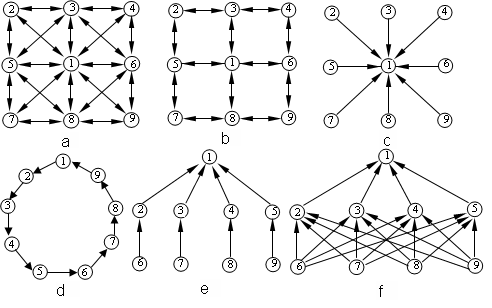
\includegraphics[width=\textwidth]{img/topology.png}
  \caption{Topológie paralelných genetických algoritmov}
  \label{img:topology}
\end{figure}
\subsection{Výsledky experimentu}
Výsledky PGA a ich interpretácia
...

%% Zaver
%%
%% Spolupráca s Petrom Javorkom
%% Spotrebovaný čas/peniaze

